\chapter{Límites y Continuidad}	
\label{Límites y Continuidad}
	\section{Introducción}
	
		

	En este tema vamos a estudiar, con algún detalle, el importante concepto teórico que es el de \emph{continuidad}. Para motivar la definición que vamos a dar de continuidad, consideremos una ley física de la forma $T = f (l )$, que relaciona los valores de una variable independiente $l$ (la longitud de la cuerda de un péndulo) con otra variable dependiente $T$ (el periodo o tiempo en dar una oscilación completa).Si queremos usar dicha ley, hemos de medir un valor $l_0$ de la variable $l$ , y es inevitable que al hacerlo cometamos algún error el cual, naturalmente, influye en el correspondiente valor de $T$, que ya no será exactamente igual a $T_0 = f(l_0)$. Surge así la pregunta natural: ?`de qué forma el error en la medida de $l$ afecta al valor resultante de $T$ ? Es claro que si para valores de $l$ muy próximos a $l_0$ obtengo valores de $T$ muy diferentes entre sí, la ley `$f$' que relaciona $l$ con $T$ no tendrá ninguna utilidad práctica.

	Puesto que los errores de medida son inevitables, no es razonable tratar de obtener el verdadero valor $T_0$. Lo que sí puede hacerse es fijar una cota de error admisible para $T$ (la cual dependerá de cada situación concreta), llamemos $\varepsilon$ (épsilon) a dicha cota, $\varepsilon > 0$, y tratar de obtener otra cota de error $\delta$ (delta) $\delta > 0$, de tal forma que siempre que midamos $l_0$ con un error menor que $\delta$ tengamos la seguridad de que el valor resultante para $T$ se diferencie de $T_0$ en menos que $\varepsilon$. Esto es, $|f(l )-f(l_0)|=|T-T_0| < \varepsilon$ siempre que $|l-l_0| < \delta$. Cuando esto efectivamente pueda hacerse para cualquier cota de error $\varepsilon > 0$ diremos que la ley `$f$'  es continua en $l_0$.

	Cabe esperar que la cota de error $\delta$ dependa del $\varepsilon$ fijado en cada caso. Intuitivamente, cuanto más pequeño sea el error permitido en los datos finales, tanto mejor tendremos que medir la variable independiente. En general, la precisión $\delta$  con la que debemos medir $l_0$ para obtener un error final menor que $\varepsilon$, depende no solamente del valor fijado de $\varepsilon$ sino también del valor de $l_0$. Esto es fácil de entender, no es lo mismo medir una longitud de varios metros que otra de unos pocos milímetros, la precisión de nuestra medida debe ser mejor en este último caso.

\textcolor{gris}{La fórmula física que describe el periodo del péndulo físico es $T=k\; \sqrt{l}\; \quad k=\frac {1}{2\pi \sqrt{g} }=cte; (g text{ es la aceleración de la gravedad})$}

	Las ideas anteriores conducen, de forma natural, a la definición matemática de continuidad. En todo lo que sigue, la letra $A$ representará un conjunto no vacío de números reales. En la práctica $A$ será siempre un intervalo o una unión de intervalos. Recuérdese que la notación $f : A \to \mathbb R$ quiere decir que $f$ es una función real cuyo dominio es $A$. Es muy importante advertir que $A$ no tiene por qué coincidir con el dominio natural de la función. Esto es así porque con frecuencia estamos interesados en estudiar propiedades de una función en una parte de su dominio natural. Además, la continuidad de $f$ depende tanto de la `regla que la define' como del conjunto en donde estamos trabajando. 
	
	Toda la idea de función continua se basa en el concepto fundamental de \emph{límite}, que desarrollamos a continuación.
	
	
	\section{Límite de una función en un punto}
	
	Empezaremos con una definición \emph{informal} de límite y daremos, más tarde, la definición formal.
	
	\begin{defi}
	
	Sea $f(x)$ una función definida en un intervalo abierto alrededor de $x_0$, excepto, posiblemente, en el propio $x_0$. Si ocurre que $f(x)$ se aproxima tanto como queramos a $L$ a medida que estemos lo suficientemente cerca de $x_0$, diremos que \textit{el límite de $f(x)$ es $L$ cuando $x$ se acerca, o tiende, a $x_0$} y lo denotaremos así:
	
	\begin{equation}
		\underset { x\rightarrow x_0 }{ lim } {f(x)}=L
	\end{equation}
		
	\end{defi}

	
	Con esta definición \emph{informal} queremos decir que $f(x)$ se acerca al número $L$ tanto como queramos, sin más que tomar valores $x$ lo suficientemente cerca de $x_0$ (por cualquiera de sus lados). Veamos un ejemplo:
	
	\begin{ejem}
		Estudia $\quad \underset { x\rightarrow 1 }{ lim } \; {\dfrac {x^2-1}{x-1}}$
	\end{ejem}
	
	Para ello vamos a construir dos sucesiones que se vayan aproximando a $1$ por cada lado, con números mayores que $1$ ($1^+$, nos acercamos a $1$ por su derecha) y con números menores que $1$ ($1^-$, nos acercamos a $1$ por su izquierda) y observemos que hace la función a medida que nos acercamos más y más a $1$.
	
	
	\begin{table}[H]
	\centering
	\begin{tabular}{l|lll|l}
	\multicolumn{1}{c|}x{} & \multicolumn{1}{c}f(x){} & \multicolumn{1}{c}{} & \multicolumn{1}{c|}x{} &  f(x)
	
	\\ \cline{1-2} \cline{4-5} 
       
         $0.9$&$1.9$&    $\qquad \qquad$      &$1.1$&$2.1$   \\
         $0.99$&$1.99$&        &$1.01$&$2.01$    \\
         $0.999$&$1.999$&      &$1.01$&$2.01$      \\
         $...$&$...$&          &$...$&  $...$      \\
         $\to 1^-$&$\to 2$&    &$\to 1^+$&$\to 2$   \\
                     
	\end{tabular}
	\end{table}
	
	Decimos que $\quad \underset { x\rightarrow 1 }{ lim } \; {\dfrac {x^2-1}{x-1}} = 2$ queriendo indicar que $f(x)$ se aproxima a $2$ cada vez que $x$ se acerca a $1$ y esto es independiente del valor que tenga $f(1)$, que en este caso no existe.
	
	En algunas ocasiones se puede calcular  $\quad \underset { x\rightarrow x_0 }{ lim } {f(x)}$ calculando $f(x_0)$ y esto ocurre cuando no se produce una \emph{indeterminación}, algo que no sabemos calcular. Ya veremos que son y como reaccionar ante una de estas  \emph{indeterminaciones}. Por ejemplo, en el caso anterior, si queremos calcular  $\quad \underset { x\rightarrow 3 }{ lim } \; {\dfrac {x^2-1}{x-1}}$, basta con calcular $f(3)=4$, ya que en este caso, el cálculo de $f(3)$ no nos ha provocado ninguna indeterminación, si hubiésemos aplicado el método anterior de ir aproximándonos a $3$ por la izquierda y la derecha hubiésemos obtenido que el límite era $f(3)=4$. No ocurría lo mismo en el caso anterior, si deseamos calcular $f(1)$ obtendremos $\frac 0 0$, cuyo valor nos resulta desconocido (\emph{indeterminación}).
	
	
	\subsection{Límites laterales}
	
	
	Sea $x_0 \in \mathbb R$, para estudiar el $ \underset { x\rightarrow x_0}{ lim } \; {f(x)}$, si se obtiene límite $\infty$ o bien $x_0$ es el nexo de una función definida a trozos (punto en el que cambia la característica o fórmula de la función a la izquierda o derecha de $x_0$) estudiaremos los límites laterales, y además,
	
	\begin{equation}	
	\exists \underset {x\to x_0}{lim}{f(x)} \leftrightarrow \exists \underset {x\to x_0^+}{lim}{f(x)} \; \wedge \;  \exists \underset {x\to x_0^-}{lim}{f(x)} \; \mbox { y } \;   \underset {x\to x_0^+}{lim}{f(x)}= \underset {x\to x_0^-}{lim}{f(x)}
	\end{equation}
	
	 \emph{`El límite, si existe, es único'}
	
	\subsection{Límites infinitos}
	
	Continuamos con una definición, también informal de momento, de lo que entendemos por límite infinito de una función en un punto.
	
	\begin{defi}
	
	Sea $f(x)$ una función definida en un intervalo abierto alrededor de $x_0$, excepto, posiblemente, en el propio $x_0$. Si ocurre que $f(x)$ toma cada vez valores más y más grandes  a medida que estemos lo suficientemente cerca de $x_0$, diremos que \textit{el límite de $f(x)$ cuando $x$ se acerca, o tiende, a $x_0$} es $+\infty$ y lo denotaremos así:
	
	\begin{equation}
		\underset { x\rightarrow x_0 }{ lim } {f(x)}=+\infty
	\end{equation}
	
	Análogamente, diremos que $f(x)$ una función definida en un intervalo abierto alrededor de $x_0$, excepto, posiblemente, en el propio $x_0$, si ocurre que $f(x)$ toma cada vez valores más y más grandes pero negativos a medida que estemos lo suficientemente cerca de $x_0$, diremos que \textit{el límite de $f(x)$  cuando $x$ se acerca, o tiende, a $x_0$} es $-\infty$ y lo denotaremos así:
	
	\begin{equation}
		\underset { x\rightarrow x_0 }{ lim } {f(x)}=-\infty
	\end{equation}
		
	\end{defi}
	
	\begin{ejer}
		Estudia $\quad \underset { x\rightarrow 1 }{ lim } \; {\dfrac {1}{x-1}}$
	\end{ejer}

	
	Para ello vamos a construir dos sucesiones que se vayan aproximando a $1$ por cada lado, con números mayores que $1$ ($1^+$) y con números menores que $1$ ($1^-$) y observemos que hace la función a medida que nos acercamos más y más a $1$.
	
	
	\begin{table}[H]
	\centering
	\begin{tabular}{l|lll|l}
	\multicolumn{1}{c|}x{} & \multicolumn{1}{c}f(x){} & \multicolumn{1}{c}{} & \multicolumn{1}{c|}x{} &  f(x)
	
	\\ \cline{1-2} \cline{4-5} 
       
         $0.9$&$-10$&    $\qquad \qquad$      &$1.1$&$10$   \\
         $0.99$&$-100$&        &$1.01$&$100$    \\
         $0.999$&$-1000$&      &$1.01$&$1000$      \\
         $...$&$...$&          &$...$&  $...$      \\
         $\to 1^-$&$\to -\infty $&    &$\to 1^+$&$\to \infty$   \\
                     
	\end{tabular}
	\end{table}
	
	Decimos que $\quad \underset { x\rightarrow 1^- }{ lim } \; {\dfrac {1}{x-1}} = -\infty$ queriendo indicar que $f(x)$ se aproxima a $-\infty$ cada vez que $x$ se acerca a $1^-$ y esto es independiente del valor que tenga $f(1)$, que en este caso no existe. Análogamente, decimos que $\quad \underset { x\rightarrow 1^+ }{ lim } \; {\dfrac {1}{x-1}} = +\infty$ queriendo indicar que $f(x)$ se aproxima a $+\infty$ cada vez que $x$ se acerca a $1^+$ . Abusando del lenguaje, podemos decir que $\quad \underset { x\rightarrow 1 }{ lim } \; {\dfrac {1}{x-1}} = \infty$, sin especificar el signo con el cual la función diverge a $\infty$. Si por ambos lados ocurre que el límite diverge a $+\infty$ o $-\infty$ sí podemos precisar que $\quad \underset { x\rightarrow x_0}{ lim } \; {f(x)} = +\infty \quad $ ó $\quad \underset { x\rightarrow x_0}{ lim } \; {f(x)} = -\infty$

	

	
	\section{Límites en el infinito}
	
	 \begin{defi}.
	 
	 Decimos que $\underset {x \to \pm \infty}{lim}{f(x)}= L$ si para toda sucesión de originales $x$ que diverjan a $\infty$, los valores que va tomando $f(x)$ se aproximan más y más a $L$
	 
	 Decimos que $\underset {x \to \pm \infty}{lim}{f(x)}= \pm \infty$ si para toda sucesión de originales $x$ que diverjan a $\infty$, los valores que va tomando $f(x)$ se aproximan más y más a $\pm \infty$
	 
	 \begin{equation}
	 	\underset {x\to \pm \infty}{lim}{f(x)}=L \quad \mbox{o} \quad \underset {x\to \pm \infty}{lim}{f(x)}=\pm \infty
	 \end{equation}

	 	
	 \end{defi}

	\vspace{2mm} Los límites en el infinito requieren un tratamiento distinto a los límites de una función en un punto:
	
	\begin{itemize}
		\item [*] Las funciones polinómicas tienen límite infinito en el infinito, el signo lo determina el signo del coeficiente del término dominante del polinomio.
		\item [*] Para funciones racionales (cocientes de polinomios), si el grado del numerador es superior al del denominador, el límite es infinito. Si el denominador es el que posee grado mayor al denominador, el límite es cero. En el caso en que numerador y denominador sean del mismo grado, el límite en el infinito es el cociente de los coeficientes de los términos dominantes (del mismo grado) de numerador y denominador.
		\item ORDEN DE INFINITOS: 
		
		\hspace{10mm} $a>1;\; n>0; \; b>1:\; \mbox{ si } x \to \infty: \quad a^x>>x^x>>log_bx$
		\item Para calcular $\underset {x \to -\infty}{lim}{f(x)} = [\mbox{cambio } x=-t] =\underset {t \to +\infty}{lim}{f(-t)}$
	\end{itemize}
	
	 NOTA: cuando al calcular un límite la función se acerca a un número real $L$, decimos que $f(x)$ \emph{converge} a $L$. Si la función se aleja al $\infty$, decimos que $f(x)$ \emph{diverge} a $\infty$.

	
	 Veamos algunos ejemplos:
	
	\begin{ejem}Ejemplos de límites en el $\infty$.
	\begin{multicols}{2}
	\begin{itemize}
		\item $\underset {x \to \infty }{lim}{3x^2-4x^5+5x-2}=-\infty  $
		\item $\underset {x \to \infty }{lim}{\frac {3x^2-1}{3-2x^2}}=\frac {3}{-2}=-\frac 3 2  $
		\item $\underset {x \to \infty }{lim}{\frac {3x^2-1}{3x^4-2x^2}}=0$
		\item $\underset {x \to \infty }{lim}{\frac {3x^2-1}{3-2x}}=-\infty$ (denominador negativo)
		\item $\underset {x \to \infty }{lim}{x^3-e^x}=-\infty$ ($e^x>>x^3$, para $x>>1$)
	\end{itemize}	
	\end{multicols}
	\end{ejem}
	
	

	 
	\section{Límites a partir de gráficas}
	
		\begin{ejem} Calcula los límites de $f(x)$ cuando $x$ tiende a $0$, $2$ y $4$ a partir de la siguiente gráfica.
		
	    \begin{multicols}{2}
	    
		\begin{figure}[H]
			\centering
			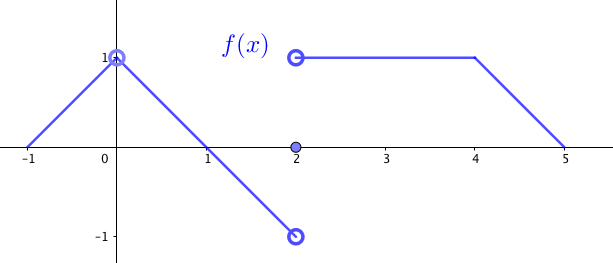
\includegraphics[width=0.5
			\textwidth]{imagenes/imagenes03/T03IM01.png}
		\end{figure}
		
		\begin{itemize}
			\item $\underset { x\rightarrow 0}{ lim } {f(x)}=1; \qquad \nexists f(1)$
			\item $\nexists \underset { x\rightarrow 2}{ lim } {f(x)}\text{:} \;  \underset { x\rightarrow 2-}{ lim } {f(x)}=-1; $
			
			$  \underset { x\rightarrow 2^+}{ lim } {f(x)}=1; \qquad  f(2)=0$
			\item $\underset { x\rightarrow 4}{ lim } {f(x)}=1; \qquad f(4)=1$
		\end{itemize}
	
	   \end{multicols}
	   
	   \end{ejem}
	   
	   \begin{ejem} Calcula los límites de $f(x)$ a partir de la siguiente gráfica, en los puntos $\{-4, -2, 0, 1, 3, 5, 7, 8, 10 \}$ y en $\pm \infty$.
	   
	   \begin{figure}[H]
			\centering
			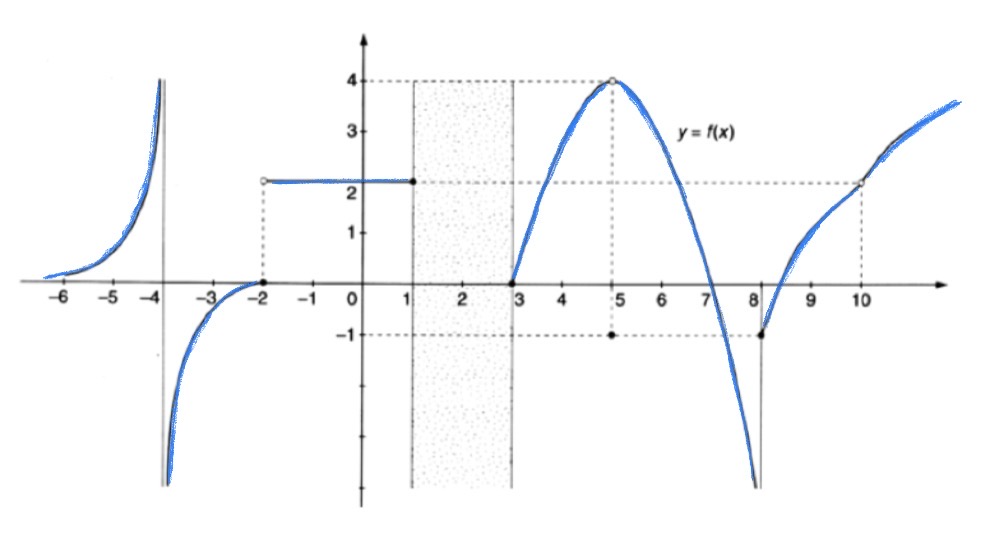
\includegraphics[width=.95
			\textwidth]{imagenes/imagenes03/T03IM02.png}
		\end{figure}
	   	
	   	\begin{itemize}
	   		\item $\underset {x \to -4^-} {lim} {f(x)}= +\infty; \quad \underset {x \to -4^+} {lim} {f(x)}=-\infty; \quad \nexists f(-4) $
	   		\item $\underset {x\to -2^-} {lim} {f(x)}=0; \quad \underset {x \to -2^+} {lim} {f(x)}=2; \quad f(2)=0$
	   		\item $\underset {x \to 0} {lim} {f(x)}=2; \quad f(0)=2$
	   		\item $\underset {x \to 1^- } {lim} {f(x)}=2; \quad \nexists \underset {x \to 1^+} {lim} {f(x)}; \quad f(1)=2$
	   		\item $\nexists \underset {x \to 3^-} {lim} {f(x)}; \quad \underset {x \to 3^+ } {lim} {f(x)}= 0; \quad f(3)=0 $
	   		\item $\underset {x \to 5} {lim} {f(x)}=4; \quad f(5)=-1$
	   		\item $\underset {x \to 7} {lim} {f(x)}=0; \quad f(7)=0$
	   		\item $\underset {x \to 8^-} {lim} {f(x)}=-\infty; \quad \underset {x \to 8^+} {lim} {f(x)}=-1; \quad f(8)=-1$
	   		\item $\underset {x \to 10} {lim} {f(x)}=2; \quad \nexists f(10)$
	   		\item $\underset {x \to -\infty}{lim}{f(x)}=0; \quad \underset {x \to \infty}{lim}{f(x)}=+\infty$
	   	\end{itemize}
	   	
	   \end{ejem}

	   \begin{ejem} Funciones exponencial y logarítmica.
	   	
	   	\begin{multicols}{2}
	    
			\begin{figure}[H]
			\centering
			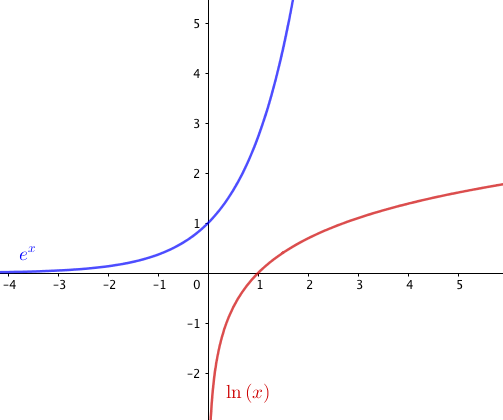
\includegraphics[width=0.3
			\textwidth]{imagenes/imagenes03/T03IM03.png}
			\end{figure}
		
			\begin{itemize}
			\item $\underset {x \to -\infty}{lim}{e^x}=0$
			\item $\underset {x \to +\infty}{lim}{e^x}=+\infty$
			\item $\underset {x \to 0^+}{lim}{\ln x}=-\infty$
			\item $\underset {x \to +\infty}{lim}{\ln x}=+\infty$
			\end{itemize}
	
	   \end{multicols}
	   	
	   \end{ejem}



		\begin{ejem}.
	   	
	   	\begin{multicols}{2}
	    
			\begin{figure}[H]
			\centering
			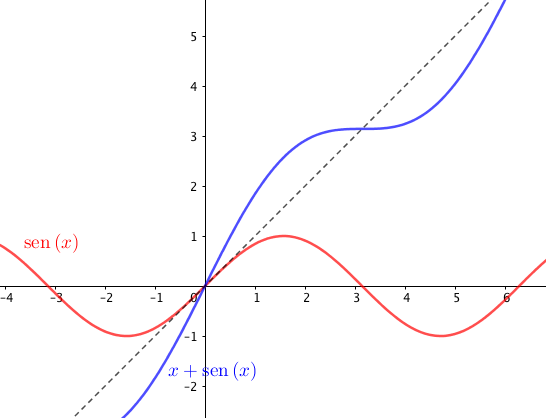
\includegraphics[width=0.4
			\textwidth]{imagenes/imagenes03/T03IM04.png}
			\end{figure}
		
			\begin{itemize}
			\item $\nexists \underset {x \to -\infty}{lim}{\sin x}$
			\item $\nexists \underset {x \to +\infty}{lim}{\sin x}$
			\item $\underset {x \to -\infty}{lim}{(x+\sin x)}=-\infty$
			\item $\underset {x \to +\infty}{lim}{(x-\sin x)}=+\infty$
			\end{itemize}
	
	   \end{multicols}
	   	
	   \end{ejem}.
	   
	   
	   \begin{ejem}.
	   	
	   	\begin{figure}[H]
			\centering
			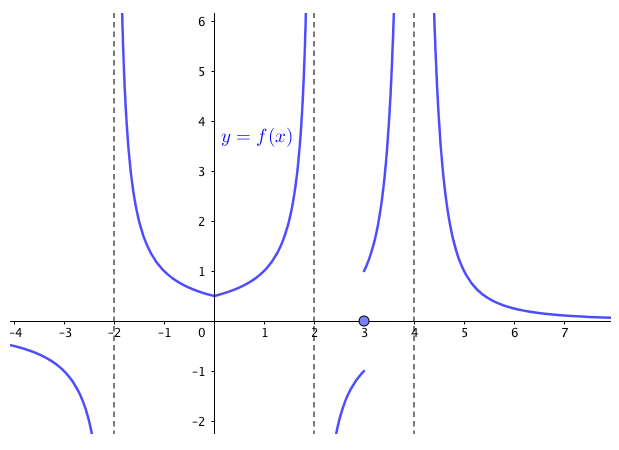
\includegraphics[width=0.8
			\textwidth]{imagenes/imagenes03/T03IM05.png}
			\end{figure}
		
	   	 	\begin{multicols}{2}
	   	 		\begin{itemize}
	   	 			\item $\underset {x\to -\infty}{lim}{f(x)}=0  $
	   	 			\item $\underset {x\to -2^{\mp}}{lim}{f(x)}=\mp \infty  $
	   	 			\item $\underset {x\to 0}{lim}{f(x)}=1/2=f(0)  $
	   	 			\item $\underset {x\to 2^{\mp}}{lim}{f(x)}=\pm \infty  $
	   	 			\item $\underset {x \to 3^{\mp}}{lim}{f(x)}=\mp 1; ;\ f(3)=0  $
	   	 			\item $\underset {x\to 4^{\mp}}{lim}{f(x)}=+\infty  $
	   	 			\item $\underset {x\to +\infty}{lim}{f(x)}=0  $
	   	 		\end{itemize}	
	   	 	\end{multicols}

	   \end{ejem}
	   
	   \section{Álgebra de límites. Indeterminaciones}
	   
		El siguiente teorema (que daremos sin demostración) nos enseña como calcular límites en un punto de funciones que son combinaciones aritméticas de otras funciones cuyos límites, en esos puntos, conocemos (siempre que no lleguemos a una \emph{indeterminación}).
		
		\begin{teor}{Álgebra de límites. }
		
		Sean $L, M, x_0, k \in \mathbb R \quad $, con $\quad \underset {x \to x_0}{lim}{f(x)}=L; \; \underset {x \to x_0}{lim}{g(x)}=M \quad \Rightarrow$
		
		\begin{itemize}
			\item [*] `El límite de la suma (de dos funciones) es la suma de los límites'.
			
				$\underset {x\to x_0}{lim}{(f(x)+g(x))}=\underset {x\to x_0}{lim}{f(x)}+\underset {x\to x_0}{lim}{g(x)}=L+M$
			\item [*]`El límite de la resta es la resta de los límites'.
			
				$\underset {x\to x_0}{lim}{(f(x)-g(x))}=\underset {x\to x_0}{lim}{f(x)}-\underset {x\to x_0}{lim}{g(x)}=L-M$
			\item [*]`El límite del producto es el producto de los límites'.
						
				$\underset {x\to x_0}{lim}{(f(x)\cdot g(x))}=\underset {x\to x_0}{lim}{f(x)} \cdot \underset {x\to x_0}{lim}{g(x)}=L\cdot M$

			\item [*]`El límite del producto de una constante por una función es el producto de la constante por el límite de la función'.
						
				$\underset {x\to x_0}{lim}{(k\cdot f(x))}=k\cdot \underset {x\to x_0}{lim}{f(x)}=k\cdot L$
				
			\item [*]`El límite del cociente es el cociente de los límites, siempre que el denominador no sea cero'.
						
				$\underset {x\to x_0}{lim}{\dfrac {f(x)} {g(x)}}= \dfrac {\underset {x\to x_0}{lim}{f(x)}} {\underset {x\to x_0}{lim}{g(x)}}=\dfrac L M; \quad M\neq 0$
				
				\item [*]`El límite de la potencia es la potencia de los límites' (siempre que no se produzca indeterminación).
						
				$\underset {x\to x_0}  {lim} { \left( f(x) ^ {g(x)} \right) } = \underset {x \to x_0}{lim}{f(x)} ^ { \underset {x \to x_0}{lim}{g(x)}  } = L^M$
				
				\end{itemize}
				
				Nota: todas estas propiedades también se cumplen cuando $x\to \pm\infty$
			
		\end{teor}
		
			\textbf{Indeterminaciones:} Llamamos \emph{indeterminación} a una expresión algebraica cuyo resultado nos es desconocido, surgen al aplicar el álgebra de límites  y obtener uno de estos $7$ resultados (\textit{indeterminaciones}):
				
				\begin{equation}
					\infty - \infty; \quad \infty \cdot 0; \quad \frac 0 0; \quad \frac {\infty}{\infty}; \quad 0^0; \quad \infty ^0; \quad 1^{\infty}
						\label{indeterminaciones}
				\end{equation}
				
				Para resolver estas indeterminaciones desarrollaremos estrategias que nos permitirán encontrar su valor sin aplicar el álgebra de límites:
				 
				\begin{itemize}
					\item En cocientes de polinomios factorizaremos por Ruffini.
					\item Si aparecen raíces cuadradas usaremos el método del conjugado
					\item En las indeterminaciones con potencias tomaremos logaritmos, pues se cumple que: $\ln {\underset {x \to x_0}{ lim}{f(x)} }= \underset {x \to x_0}{lim}{\ln f(x)}$
				\end{itemize}
				
		
		 
		 ATENCIÓN: no son indeterminaciones:
		
		
			\begin{figure}[H]
			\centering
			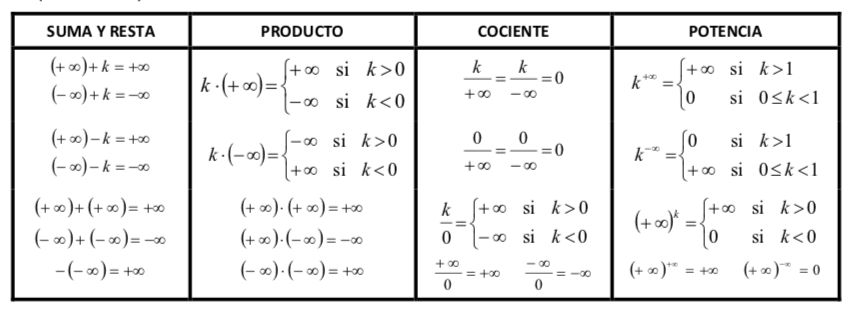
\includegraphics[width=1
			\textwidth]{imagenes/imagenes03/T03IM06.png}
			\end{figure}
	
	
	
	\section[Criterio del Sandwich y teorema de la conservación del signo $\; \divideontimes$]{Criterio del Sandwich y teorema de la conservación del signo $\; \divideontimes$}
	\sectionmark{Ths. Sandwid y conservación signo}
	
	\vspace{2mm}\begin{teor} {Teorema (criterio) del Sandwich.}
	\label{teor:Sandwich}
	Supongamos que $g(x)\le f(x) \le h(x)$ para todo $x$ en algún intervalo abierto que contenga a $x_0$, excepto posiblemente en el propio $x_0$, supongamos también que $\underset {x\to x_0}{lim}{g(x)}=\underset {x\to x_0}{lim}{h(x)}=L$, entonces: $\underset {x\to x_0}{lim}{f(x)}=L$
		
	\end{teor}
	
	\begin{ejem}.
	\label{ejem:sinx/x}
		
		\begin{multicols}{2}
			\begin{figure}[H]
			\centering
			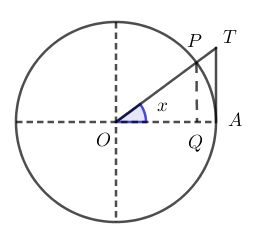
\includegraphics[width=0.4
			\textwidth]{imagenes/imagenes03/T03IM07.png}
		\end{figure}
		
		En una circunferencia de radio $1$ tomamos un ángulo $\widehat { AOP } $ de $x$ radianes. $\overline { PQ } =\sin  x; \quad \overline {TA}=\tan x; \quad $ arco $\; \widehat { PA } =x$
		
		Como $\overline {PQ}<\widehat{PA}<\overline{TA} \to \sin x < x < \tan x$
			
		Dividiendo por $\sin x \quad : 1< \dfrac {x}{\sin x}< \dfrac {1} {\cos x} \to 1> \dfrac {\sin x}{x} > \cos x$
		
		Tomando límites cuando $x\to 0: \quad 1 \ge \dfrac {\sin x}{x} \ge \cancelto {1}{\cos x} $
		
		Luego:  $\quad \underset {x\to 0}{lim}\; {\dfrac {\sin x}{x}}=1$
		\end{multicols}

		
	\end{ejem}
	
	\begin{teor}
	
	
	Si $f(x) \le g(x)$  para todo $x$ en algún intervalo abierto que contenga a $x_0$, excepto posiblemente en el propio $x_0$, y existen los límites de $f(x)$ y de $g(x)$ cuando $x\to x_0$, entonces: $\underset {x\to x_0}{lim}{f(x)} \le \underset {x\to x_0}{lim}{g(x)}$
		
	\end{teor}
	
	\begin{lema}Teorema de conservación del signo.
	\label{teor:conserva-signo}
	
	Sea $f:[a,b]\to \mathbb R$, continua en $x_o \in ]a,b[ \; \Rightarrow \mbox{ si } f(x_0)\neq 0 \to \exists \; E_{\delta}(x_0)=]x_0-\delta, x_0+\delta[ \;  / \; f(x) \mbox{ tiene el mismo signo que } f(x_0)$
		
	\end{lema}

	
	\begin{proof} Este lema (teorema) lo usaremos más tarde para la demostración del importantísimo teorema de Bolzano.
	
	Supongamos $f(x_0)>0 \to \mbox{ sea } \varepsilon>0 \;  / \; \varepsilon < f(x_0) \to 0<f(x_0)-\varepsilon<f(x_0)+\varepsilon$
	
	Como $f$ es continua en $x_0 \to \exists \; \delta>0 \; / \; \mbox { si } |x-x_0|<\delta \to |f(x)-f(x_0)|<\varepsilon$ 
	
	$-\varepsilon < f(x)-f(x_0) < \varepsilon \to 0<f(x_0)-\varepsilon<f(x)<f(x_0)+\varepsilon$
	
	Luego $f(x)>0, \; \forall x \in ]x_0-\delta, x_0+\delta[$
	
	La demostración es análoga si $f(x_0)<0$
		
	\end{proof}

	
	\section{Indeterminaciones $1^\infty,\; 0^0, \; \infty^0$}
	\label{sec-metodo-e}
	Este tipo de indeterminaciones se resuelven tomando logaritmos, pero dejaremos su resolución para capítulos posteriores, cuando veamos la \emph{Regla de L'Hôpital} en el capítulo \ref{AplicDeriv} `aplicaciones de las derivadas'. No obstante, existe un método `rápido' para las indeterminaciones $1^\infty$ que pasamos a detallar.
	
	\begin{teor}{Método del número $e$ para la indeterminación $1^\infty$}.
	\label{teor:metodo-numero-e}
	\begin{equation*}
		\mbox{si } \underset {x\to x_0}{lim}{{\left( f(x)\right)}^{g(x)} } \mbox{ presenta una indeterminación de la forma } 1^\infty \Rightarrow 
	\end{equation*}
		\begin{equation}
			\Rightarrow  \underset {x\to x_0}{lim}{{\left( f(x)\right)}^{g(x)} }=e^{\underset {x \to x_0}{lim}{(f(x)-1)\cdot g(x)}}	
		\end{equation}
	\end{teor}
	
	
	\begin{proof} La demostración consiste en transformar la expresión dada en la que define el número $e$.
	
		\begin{equation*}
		e=\underset {f(x)\to \infty}{lim} { {\left( 1+\dfrac {1}{f(x)} \right) }^{f(x)}}
		\end{equation*}
		
		Si $ \underset {x\to x_0}{lim}{{\left( f(x)\right)}^{g(x)} } $ va como $1^\infty$, vamos haciendo las siuientes transformaciones:
		
		\scriptsize{\vspace{2mm}$f(x)^{g(x)}= (1+f(x)-1)^{g(x)}=\left(1+\dfrac {1}{\dfrac {1}{(f(x)-1)}} \right)^{g(x)}=\left[  
			\left(1+\dfrac {1}{\dfrac {1}{(f(x)-1)}}\right)^{\dfrac {1}{f(x)-1}} 
			\right]^{(f(x)-1)\cdot g(x)}\quad $ } \normalsize
		
		Tomando límites cuando $x \to x_0$, Como $f(x)\to 1$, el límite del corchete es, por definición, el número $e$, así que tendríamos la expresión que queríamos demostrar:
		
		\begin{equation*}
			 \underset {x\to x_0}{lim}{{\left( f(x)\right)}^{g(x)} }=[1^\infty]=e^{\underset {x \to x_0}{lim}{(f(x)-1)\cdot g(x)}}	
		\end{equation*}
		 
		
	\end{proof}
	
	\section{Ejercicios de cálculo de límites}
	\subsection{Ejercicios resueltos de límites}	
	
	
	\begin{ejre} Calcula: $\quad \underset {x\to 1}{lim}\; { \frac {x^2+x-2}{x^2-x}}$
	
	\end{ejre}
	
	\begin{proofw}\renewcommand{\qedsymbol}{$\diamond$}
	
		$\underset {x\to 1}{lim}{ \frac {x^2+x-2}{x^2-x}}=\frac 0 0; \; $ indeterminación. Factorizaremos (Ruffini) el numerador y {denominador}:
		$\quad \underset {x\to 1}{lim}{ \frac {x^2+x-2}{x^2-x}}=
		\underset {x\to 1}{lim}{ \frac {\cancel{(x-1)}(x+2)}{\cancel{(x-1)}x}} = \underset {x\to 1}{lim}{\frac {x+2}{x}}=\frac 3 1 = 3$
	\end{proofw}
	
	\begin{ejre} Calcula: $\quad \underset {x\to 0}{lim}\; {\dfrac {\sqrt{x^2+100}-10}{x^2}}$
		
	\end{ejre}
	
	\begin{proofw}\renewcommand{\qedsymbol}{$\diamond$}

	$\quad \underset {x\to 0}{lim}{\dfrac {\sqrt{x^2+100}-10}{x^2}}=\frac 0 0\quad$ Indeterminación, aparecen raíces cuadradas, usaremos la \emph{técnica del conjugado}, multiplicar y dividir la expresión dada por la expresión conjugada de aquella donde aparece la raíz cuadrada:
	
	$\quad \underset {x\to 0}{lim}{\dfrac {\sqrt{x^2+100}-10}{x^2}}= \underset {x\to 0}{lim}{\dfrac {\sqrt{x^2+100}-10}{x^2}}\cdot \dfrac{\sqrt{x^2+100}+10}{\sqrt{x^2+100}+10} = \underset {x\to o}{lim}{\dfrac {x^2+100-100}{x^2\; (\sqrt{x^2+100}+10)}}= 
	\underset {x\to 0}{lim}{\dfrac {\cancel{x^2}}{\cancel{x^2}\; (\sqrt{x^2+100}+10)}}=\underset {x\to 0}{lim}{\dfrac 1 {\sqrt{x^2+100}+10}}=\dfrac 1 {10+10}=\dfrac 1 {20}$ 
	\end{proofw}
	
	\begin{ejre} Calcula: $\quad \underset {x \to -2}{lim}\; {\dfrac {x^2-4}{x^2+4x+4}} $
		
	\end{ejre}
	\begin{proofw}\renewcommand{\qedsymbol}{$\diamond$}
	
	$\quad \underset {x \to -2}{lim}{\dfrac {x^2-4}{x^2+4x+4}} = \frac 0 0\; $ (indeterminado, factorizamos) 	
	$= \underset {x \to -2}{lim}{\dfrac {(x-2) \cancel{(x+2)}}{(x+2)^ {\cancel{2}}}} = \underset {x \to -2}{lim} {\dfrac {x-2}{x+2}} = \dfrac {-4}{0}=\infty $  

	\end{proofw}
	
	Nota: en adelante, ante la presencia de un límite infinito no estudiaremos los límites laterales (diremos que se trata de un límite $\infty$ sin especificar el signo) pues, aunque dan mucha información, en temas futuros estudiaremos la derivada de una función y el estudio de su signo nos proporcionará la información que ahora obviamos. 
	
	\begin{ejre} Calcula: $\quad \underset {x \to 3}{lim}\; \left({\dfrac {x}{x-3} \cdot \dfrac {x^2-9}{x+1}}\right)$	
	\end{ejre}
	
	\begin{proofw}\renewcommand{\qedsymbol}{$\diamond$}
	
	$\underset {x \to 3}{lim}\; \left({\dfrac {x}{x-3} \cdot \dfrac {x^2-9}{x+1}}\right)=[\infty \cdot 0]= \underset {x\to 3}{lim}{\dfrac {x(x+3)\cancel{(x-3)}}
		{\cancel{(x-3)}(x+1)}}=\dfrac {18} 4=\dfrac 9 2$
	\end{proofw}
	
	\begin{ejre} Calcula $\quad \underset {x \to 3} {lim} \; {\dfrac {3x-x^2}{3-\sqrt {3x}}}$	
	\end{ejre}
	
	\begin{proofw}\renewcommand{\qedsymbol}{$\diamond$}
	
	$\underset {x \to 3} {lim} \; {\dfrac {3x-x^2}{3-\sqrt {3x}}}=[ 0 / 0]= \underset {x \to 3}{lim} { \dfrac {x(3-x)(3+\sqrt{3x})} {(3-\sqrt
	3x)(3+\sqrt
	3x)} }= \underset {x \to 3}{lim} { \dfrac {x\cancel{(3-x)}(3+\sqrt{3x})} {3\cancel{(3-x)}} }=6$	
	\end{proofw} 
	
	\begin{ejre} Calcula: $\quad \underset {x \to \infty}{lim}\; \left( {\dfrac {6x^2-1}{3x+2} - \dfrac {4x^2+2x}{2x-2}} \right)$
		
	\end{ejre}
	
	\begin{proofw}\renewcommand{\qedsymbol}{$\diamond$}

	 $\underset {x \to \infty}{lim}\; \left( {\dfrac {6x^2-1}{3x+2} - \dfrac {4x^2+2x}{2x-2}} \right)=[\infty -\infty]= $
	 
	 $\underset{x\to \infty}{lim}{\dfrac {(6x^2-1)(2x-2)-(4x^2+2x)(3x+2)}{(3x+2)(2x-2)}}=\underset{x\to \infty}{lim}{\dfrac {-26x^2+\cdots}{6x^2+\cdots}}=\frac {-13}{3}$
	\end{proofw}
	
	\begin{ejre} Calcula: $\quad \underset {x \to \infty}{lim}\; {\dfrac {e^x+1}{x^2+\ln x}}$
		
	\end{ejre}
	
	\begin{proofw}\renewcommand{\qedsymbol}{$\diamond$}

	$\underset {x \to \infty}{lim}\; {\dfrac {e^x+1}{x^2+\ln x}}=[e^x>>x^2]=+\infty$
	\end{proofw}
	
	
	\begin{ejre}Calcula $\quad \underset {x \to \infty}{lim}\; {(\sqrt{x^2-2x+1}-x+3)}$
		
	\end{ejre}
	
	\begin{proofw}\renewcommand{\qedsymbol}{$\diamond$}

	 $\underset {x \to \infty}{lim}\; {(\sqrt{x^2-2x+1}-x+3)}=[\infty - \infty]=$
	 
	 $=\underset {x \to \infty}{lim}\; {(\sqrt{x^2-2x+1}-(x-3))}\cdot \dfrac{(\sqrt{x^2-2x+1}+(x-3))}{(\sqrt{x^2-2x+1}+(x-3))}=$
	 
	 $=\underset{x\to \infty}{lim}{\dfrac {4x-8}{(\sqrt{x^2-2x+1}+(x-3))}}=\dfrac {4}{\sqrt{1}+1}=\dfrac 4 2=2$
	\end{proofw}
	
	\begin{ejre} Calcula: $\quad \underset {x \to\infty }{lim}\; {\dfrac {2x}{\sqrt{x^2+3x+4}-x}}$
		
	\end{ejre}
	
	\begin{proofw}\renewcommand{\qedsymbol}{$\diamond$}

	$\underset {x \to\infty }{lim}\; {\dfrac {2x}{\sqrt{x^2+3x+4}-x}}=[\mbox{mayor potencia de }x]=\dfrac {2}{\sqrt{1}-1}=\dfrac 2 0=\infty$
	\end{proofw}
	
	\begin{ejre}Calcula: $\quad \underset {x \to \infty}{lim}\; {\dfrac {\sqrt{2x^4-3x+1}-5x^2+1}{\sqrt {x^2-x+1}+3\sqrt{x^4-1}}}$
		
	\end{ejre}
	
	\begin{proofw}\renewcommand{\qedsymbol}{$\diamond$}

	$\underset {x \to \infty}{lim}\; {\dfrac {\sqrt{2x^4-3x+1}-5x^2+1}{\sqrt {x^2-x+1}+3\sqrt{x^4-1}}}=[\mbox{mayor potencia de }x]=$
	
	$=\underset {x\to \infty}{lim}{\dfrac {\sqrt{2}(x^2)-5(x^2)} {3(x^2)}}=\dfrac {\sqrt{2}-5}{3}$
	\end{proofw}
	
	
	\begin{ejre}Calcula: $\quad \underset{x \to  -\infty}{lim}\; {(\sqrt{
	x^2-2x+4}+x)}$
		
	\end{ejre}
	
	\begin{proofw}\renewcommand{\qedsymbol}{$\diamond$}

	$\underset{x \to  -\infty}{lim}\; {(\sqrt
	{x^2-2x+4}+x)}=[x=-t]=\underset{t \to  +\infty}{lim}\; {(\sqrt
	{t^2+2t+4}-t)}=[\infty- \infty]=$
	
	$=\underset{t \to  +\infty}{lim}\; {(\sqrt
	{t^2+2t+4}-t)}\cdot \dfrac {(\sqrt
	{t^2+2t+4}+t)}{(\sqrt
	{t^2+2t+4}+t)}=$
	
	$=\underset {t\to +\infty}{lim}{\dfrac {2t+4}{\sqrt{t^2+2t+4}+t}}=\frac {2}{1+1}=1$
	\end{proofw}
	
	
	\begin{ejre}Calcula: $\quad \underset{x \to \pm \infty}{lim}\; {\dfrac {\sqrt{x^2-2x}}{x}}$
		
	\end{ejre}
	
	\begin{proofw}\renewcommand{\qedsymbol}{$\diamond$}

	 $\quad \underset{x \to +\infty}{lim}\; {\dfrac {\sqrt{x^2-2x}}{x}}=\dfrac 1 1 = 1$
	 
	  $\quad \underset{x \to  -\infty}{lim}\; {\dfrac {\sqrt{x^2-2x}}{x}}=[x=-t]=\underset {t\to +\infty}{lim}{\dfrac {\sqrt{t^2+2t}}{-t}}= \dfrac 1 {-1}=-1$
	\end{proofw}
	
	\begin{ejre}Calcula: $\quad \underset{x\to 2}{lim}\; {\left(\dfrac {2x^2-x-1}{7-x}\right)^{\dfrac {1}{x-2}}}$
		
	\end{ejre}
	
	\begin{proofw}\renewcommand{\qedsymbol}{$\diamond$}

	$\underset{x\to 2}{lim}\; {\left(\dfrac {2x^2-x-1}{7-x}\right)^{\dfrac {1}{x-2}}}=[1^\infty]=exp \left\{ 
		\underset {x\to 2}{lim}
		{\left (\dfrac {2x^2-x-1}{7-x} -1 \right)\cdot \dfrac {1}{x-2}}
		\right\}=$
		
		$= exp \left\{\underset {x\to 2}{lim}
		{\dfrac {2x^2-8}{7-x} \cdot \dfrac {1}{x-2}}
		\right\}=
		exp 
		\left\{ 
		\dfrac {2(x+2)\cancel{(x-2)}} {(7-x)\cancel{(x-2)}}  
		\right\} 
		=e^{\frac 8 5}$
	\end{proofw}
	
	
	\begin{ejre}Calcula: $\quad \underset{x\to 0}{lim}\;{\dfrac {sin 3x}{2x}}$
		
	\end{ejre}
	
	\begin{proofw}\renewcommand{\qedsymbol}{$\diamond$}
	
	$\underset{x\to 0}{lim}\;{\dfrac {sin 3x}{2x}}=$[como vimos en la aplicación del criterio de Sandwich]=
	
	$=\underset {x\to 0}{lim}{ \dfrac {\sin (3x)} {\frac 2 3 \; (3x)}  }= \frac 3 2 \; \underset {x\to 0}{lim}{\dfrac {\sin (3x)}{(3x)}}= \frac 3 2 \cdot 1 = \frac 3 2$
	
	\end{proofw}
	
	\subsection{Ejercicios propuestos de cálculo de límites}
	
	\begin{multicols}{2}
	\begin{enumerate}
		\item $\underset{x\to +\infty}{lim}\;{\dfrac{3+2\sqrt{x}}{\sqrt{2x+1}}}$
		 
		\rightline{\textcolor{gris}{Solución: $\sqrt{2}$}}
		
		\item $\underset{x \to +\infty}{lim}\;{\left(\dfrac{x^2}{x-3}-\dfrac{x^2}{5-x}  \right)}$
		 
		\rightline{\textcolor{gris}{Solución: $-\infty$}}
		
		\item $\underset{x\to -\infty}{lim}\;{\dfrac{\sqrt{x^2-5}}{1-2x}}$
		
		\rightline{\textcolor{gris}{Solución: $1/2$}}
		
		 \item $\underset{x\to +\infty}{lim}\;{\left(\dfrac{x^2-5x}{x+1}-\dfrac{3x}{2} \right)}$
		
		\rightline{\textcolor{gris}{Solución: $-\infty$}}
		
		\item $\underset{x\to +\infty}{lim}\;{\left( x^2-\sqrt{x`4+2x} \right)}$
		
		\rightline{\textcolor{gris}{Solución: $0$}}
		
		\item $\underset{x\to \pm\infty}{lim}\;{\left(  \dfrac {3x+4}{2x+5}\right)^{x-1}}$
		
		\rightline{\textcolor{gris}{Solución: $\infty;\; 0$}}
		
		\item $\underset{x\to \infty}{lim}\;{\left( \dfrac {x^2+1}{x^2-1} \right) ^{x^2}}$
		
		\rightline{\textcolor{gris}{Solución: $e^2$}}
		
		\item $\underset{x\to +\infty}{lim}\;{\left( \dfrac {3x-4}{3x-2} \right) ^{\dfrac {x+1}{3}}}$
		
		\rightline{\textcolor{gris}{Solución: $e^{-2/9}$}}
		
		\item $\underset{x\to -\infty}{lim}\;{\left( 1-\dfrac{1}{x^2}\right)^{3x-2}}$
		
		\rightline{\textcolor{gris}{Solución: $1$}}
		
		\item $\underset{x \to -\infty}{lim}\;{\left( \dfrac {x-3}{x+2} \right) ^{x^2-5}}$
		
		\rightline{\textcolor{gris}{Solución: $+\infty$}}
		
		\item $\underset{x \to -\infty}{lim}\;{\left(\sqrt{x^2+2x}-\sqrt{x^2-4} \right)}$
		
		\rightline{\textcolor{gris}{Solución: $-1$}}
		
		\item $\underset{x\to \pm\infty}{lim}\;{\dfrac {e^x}{x^2-1}}$
		
		\rightline{\textcolor{gris}{Solución: $\infty;\; 0$}}
		
		\item $\underset{x\to \pm \infty}{lim}\;{(\sqrt{3x^2+2}-5x)}$
		
		\rightline{\textcolor{gris}{Solución: $\mp\infty$}}
		
		\item $\underset{x\to \pm \infty}{lim}\;{\dfrac {2x+3}{\sqrt{3x^2-1}}}$
		
		\rightline{\textcolor{gris}{Solución: $\pm \frac {2}{\sqrt{3}}$}}
		
		\item Calcula los límites cuando $x \to \pm \infty$ de la función: 
		
		\begin{equation*}
		f(x)=
		\begin{cases} 
		\;\;  \dfrac{1-x}{x+2} &\mbox{if } x\le 0 \\ 
		\; \dfrac {\mathrm{ln} x}{x} & \mbox{if } x>0 
		\end{cases}
		\end{equation*}
		
		\rightline{\textcolor{gris}{Solución: $0,\; -1$}}
		
		\item Calcula los límites cuando $x \to \pm \infty$ de la función: 
		
		\begin{equation*}
		g(x)=
		\begin{cases} 
		\;\;  \dfrac{2x}{\sqrt{x^2+1}} &\mbox{if } x\le 0 \\ 
		\; e^x-\mathrm{ln}x & \mbox{if } x>0 
		\end{cases}
		\end{equation*}
		
		\rightline{\textcolor{gris}{Solución: $\infty,\; -2$}}
		
		\item $\underset{x\to 1}{lim}\;{\dfrac {x^2-7x+6}{1-x}}$
		
		\rightline{\textcolor{gris}{Solución: $5$}}
		
		\item $\underset{x\to 1}{lim}\;{\dfrac {x^3-4x^2+5x-2}{(x^3-1)(x-2)}}$
		
		\rightline{\textcolor{gris}{Solución: $0$}}
		
		\item $\underset{x\to 2}{lim}\;{\dfrac {x^2+3x-10}{x^3-x^2-8x+12}}$
		
		\rightline{\textcolor{gris}{Solución: $\infty$}}
		
		\item $\underset{x\to 2}{lim}\;{\left[ \dfrac {3}{x^2-5x+6} - \dfrac{4}{x-2} \right]}$
		
		\rightline{\textcolor{gris}{Solución: $\infty$}}
		
		\item $\underset{x \to 2}{lim}\;{\dfrac {1-\sqrt{3-x}}{x-2}}$
		
		\rightline{\textcolor{gris}{Solución: $1/2$}}
		
		\item $\underset{x\to 0}{lim}\;{\dfrac {\sqrt{x+9}-3}{x^2}}$
		
		\rightline{\textcolor{gris}{Solución: $\infty$}}
		
		\item $\underset{x\to 0}{lim}\;{\dfrac {\sqrt{1+x}-\sqrt{1-x}}{3x}}$
		
		\rightline{\textcolor{gris}{Solución: $1/3$}}
		
		\item $\underset {x\to 0}{lim}\;{ \left( \dfrac{x^2+1}{2x+1} \right) ^{\dfrac 1 x} }$
		
		\rightline{\textcolor{gris}{Solución: $e^{1/2}$}}
		
		
		\item $\underset{x\to 0}{lim}\;{\dfrac {1-\cos x}{x^2}}$
		
		\rightline{\textcolor{gris}{Ayuda: multiplica y divide por $1+\cos x$}}
		
		\item $\underset{x\to \infty}{lim}\;{\dfrac {\left\lfloor x \right\rfloor }{x}}$
		
		\rightline{\textcolor{gris}{Ayuda: $x<\left\lfloor x \right\rfloor <x+1$}}
		
		\item $\underset{x\to \infty}{lim}\;{\sqrt[x]{x}}$
		
		\rightline{\textcolor{gris}{Ayuda: toma logaritmos}}
		
		\item $\underset{x\to \infty}{lim}\;{\log_{x} (x+1)}$
		
		\rightline{\textcolor{gris}{Ayuda: $x+1=x\cdot (1 + \frac 1 x)$}}
		
		\item $\underset{a\to b}{lim}\;{\dfrac {a\sqrt{a}-b\sqrt{b}}{\sqrt{a}-\sqrt{b}}}$
		
		\rightline{\textcolor{gris}{Solución: $3b$}}
		
		\item $\underset{x\to +\infty}{lim}\;{[\ln(x+1)-\ln(x)]}$
		
		\rightline{\textcolor{gris}{Solución: $0$}}
		
		\item $\underset {x\to \pm \infty}{lim}\; {(|x-3|-|x|)}$
		
		\rightline{\textcolor{gris}{Solución: $+\infty$, en ambos casos}}
		
		\item $\underset {x\to \pm \infty}{lim}\; {\dfrac {x+1}{x}}$
		
		\rightline{\textcolor{gris}{Solución: $x=\pm 1$}}
		
		\item Encuentra el valor de $a$ para que el siguiente límite sea una indeterminación $\underset {x\to -1}{lim}\; {\dfrac {ax^2+2x-6}{x^2-1}}$. Calcular el límite para ese valor de $a$.
		
		\rightline{\textcolor{gris}{Solución: $a=8; \quad$ límite $=7$ }}
		
		\item Determina el valor de $a$ para que $\underset {x\to \infty}{lim}\; { \left( \dfrac {3x-2}{3x-1} \right)^{\dfrac {ax-4}{5}} }=e^{2}$
		
		\rightline{\textcolor{gris}{Solución: $a=-30$}}
		
		\item Encuentra los valores de $a$ y $b$ para que $\underset {x\to +\infty}{lim}\;{(\sqrt{ax^2+x}-\sqrt{bx^2+3x})}=-\dfrac {\sqrt{2}}{2}$
		
		\rightline{\textcolor{gris}{Solución: $a=b=2$}}
		
	\end{enumerate}
	\end{multicols}
	
	\section{Definiciones formales de límites $\; \divideontimes$ }
	
	
	\begin{defi} \label{defi:limite} Definición (formal) de límite (finito) de una función en un punto.
	
	Sea $f(x)$ definida en un intervalo abierto alrededor de $x_0$, excepto posiblemente en el propio $x_0$. Decimos que	\textbf{límite de $f(x)$ cuando $x$ se aproxima a $x_0$ es el número L}, y escribimos:
	
	\begin{equation*}
		\underset {x\to x_0}{lim}\; {f(x)}=L
	\end{equation*}
	
	si, para cada número $\varepsilon >0$, existe un número $\delta > 0$ correspondiente, tal que para toda x,
	
	\begin{equation*}
		0<|x-x_0|<\delta \quad \Rightarrow \quad |f(x)-L|<\varepsilon
	\end{equation*}
	\end{defi}

	Cuando decíamos informalmente que el límite de $f(x)$ era $L$ cuando $x \to x_0$ queríamos decir que nos podíamos aproxminar todo lo que quisieramos a $L$, alejarnos de $L$ menos que cualquier cantidad positiva por pequeña que sea $\varepsilon>0$. Eso se traduce ahora en la expresión formal $|f(x)-L|<\varepsilon$. Para ello bastaba con tomar números lo suficientemente próximos a $x_0$ y eso lo determina ahora la cantidad $\delta(\varepsilon)>0$ del siguiente modo: $0<|x-x_0|<\delta$.
	
	
		
		
		\begin{ejem} Demuestra que $\underset {x\to 2}{lim}\;{2x-1}=3$.
		
		\begin{multicols}{2}
			\begin{figure}[H]
			\centering
			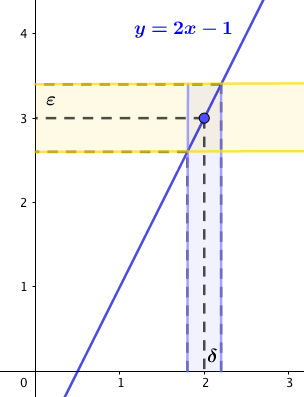
\includegraphics[width=0.2
			\textwidth]{imagenes/imagenes03/T03IM08.png}
		\end{figure}
		
		Cuando decimos que $\underset {x\to 2}{lim}\;{2x-1}=3$, queremos decir que nos podemos acercar tanto como queramos a $3$. 
		
		Si por ejemplo nos queremos acercar más que una pequeña cantidad $\varepsilon>0$, tendremos que encontrar el $\delta_{\varepsilon}$ que nos lo garantice. Así:
		\end{multicols}
		
		$|f(x)-3|=|(2x-1)-3|<\varepsilon; \quad |2x-4|<\varepsilon; \quad 2|x-2|<\varepsilon \quad \Rightarrow \quad |x-2|<\varepsilon/2=\delta$. Basta con tomar $\delta=\varepsilon/2$.
			
		

		\end{ejem}
		
		
		\begin{ejem} Comprueba, usando la definición de límite, que $\underset {x\to 1}{lim}\;{5x-3}=2$
		
			 $\underset {x\to 1}{lim}\;{5x-3}=2 \longleftrightarrow  \forall \varepsilon>0,\; \exists \delta_{\varepsilon}>0:\quad 0<|x-1|<\delta \Rightarrow |f(x)-2|<\varepsilon$
			
			$|f(x)-2|=|(5x-3)-2|=|5x-5|=5|x-1|<\varepsilon \Rightarrow |x-1|<\varepsilon/5=\delta$. 
			
			Basta tomar $\delta=\varepsilon/5$ para asegurarnos de separarnos del límite, $2$, menos que la cantidad prefijada $\varepsilon$. Si, por ejemplo quisiéramos estar a menos de $5$ millonésimas de $2$ con $f(x)$, bastaría tomar números $x$ que se alejen del $1$ menos de una millonésima.
		\end{ejem}
		
		\begin{ejem} Un ejemplo algo más complicado.
		Demuestra que $\underset{x\to 1}{lim}\;{\dfrac{2x}{2x^2-x-3}}=-1$
		
		Si $f(x)=\dfrac{2x}{2x^2-x-3} = \dfrac {2x}{(x+1)(2x-3)},\; x\neq-1; x\neq 3/2$, debemos probar que:
		
		$\forall \varepsilon>0,\; \exists \delta>0: \mbox{ si } x\in Dom(f)\sim \{ 1, -1, 3/2\}$ y si $0<|x-1|<\delta \to$ 
		
		
		\hspace{10mm}
		$\to\left| \dfrac{2x}{2x^2-x-3}-(-1) \right|<\varepsilon$
			
		 Para determinar $\delta$ en función de $\varepsilon$ partiremos de $|f(x)-L|$ para transformarla en factores que contengan a $|x-1|$ y $|g(x)|$, que deberemos acotar.
		
		 $\left| \dfrac{2x}{2x^2-x-3}+1 \right|= \left| \dfrac{(2x+3)(x-1)}{(x+1)(2x-3} \right|=\left| \dfrac{(2x+3)}{(x+1)(2x-3)} \right|\cdot |x-1|=|g(x)|\cdot|x-1|$
		
		Tenemos:  $0<|x-1|<\delta \to |g(x)|\cdot|x-1|<\varepsilon$
		
		 Ahora procederemos a la búsqueda apropiada de una $\delta$ para acotar $|g(x)|$.
		
		Como $x+1=0$ y $2x-3=0$ son dos \emph{asíntotas verticales} de la función $f$ (hacen que f se dispare al $\infty$) y siendo $x=3/2$ el punto más próximo a $x_0=1$ (el otro, $x=-1$ es más lejano), elegiremos $\delta_1=\frac 1 2 |\frac 3 2 - 1|=\frac 1 4$
		
		 Tenemos ahora que si $|x-1|<\delta<\delta_1 \to |x-1|<\frac 1 4 \leftrightarrow -\frac 1 4 < x-1 < \frac 1 4 \leftrightarrow \frac 3 4 < x < \frac 5 4$
		
		 Ahora acotaremos cada uno de los factores de $g(x)$:
		
		\begin{itemize}
		
			\item [*] $\frac 3 2 < 2x < \frac 5 2 \leftrightarrow \frac 9 2 < 2x+3 < \frac {11} {2} \to |2x+3|<\frac {11}2$
			\item [*] $\frac 3 2 < 2x < \frac 5 2 \leftrightarrow -\frac {3} 2 < 2x-3 < -\frac {11} {2} \leftrightarrow -2 < \dfrac {1}{2x-3}< -\frac {2}{3}\to \left| \dfrac {1}{2x-3} \right|<2$
			\item [*] $\frac 7 4 < x+1 < \frac 9 4 \leftrightarrow \frac 4 9 < \dfrac {1}{x+1} < \frac 4 7 \to \left| \dfrac {1}{x+1} \right| <\frac 4 7$
		\end{itemize}
		
		Entonces: $|g(x)|= \dfrac {|2x+3|}{|x+1|\cdot |2x-3|}< \frac {11}2 \cdot 2 \cdot \frac 4 7 = \frac {44} 7 \to |g(x)|<\frac {44} 7 =M$
		
		 Luego: $0<|x-1|<\delta \to \frac {44} 7 |x-1|< \varepsilon \to |x-1|<7\varepsilon/44=\delta_2$
		
		 Por tanto, eligiendo $\delta=min\{1/4,\; 7\varepsilon/44\}$ se tiene que:
		
		 $0<|x-1|<\delta \to \dfrac{|2x+3|}{|x+1|\cdot |2x-3|}<\frac {44}{7} \mbox { y } |x-1|<\frac {7\varepsilon}{44} \to $
		
		 $\to \dfrac{|2x+3|}{|x+1|\cdot |2x-3|}|x-1|<\frac {44}{7} \frac {7\varepsilon}{44}=\varepsilon$,
		
		 
		\hspace{20mm}Es decir: $ \left| \dfrac{2x}{2x^2-x-3}-(-1)  \right|<\varepsilon \qquad \qquad \qquad \qquad c.q.d.$
		\end{ejem}
		
		
		\begin{ejem} Demostración del teorema del límite de la suma visto en álgebra de límites.
		
		Sean $L, M,  \in \mathbb R \quad $, con $\quad \underset {x \to x_0}{lim}{f(x)}=L; \; \underset {x \to x_0}{lim}{g(x)}=M \quad \Rightarrow$

		
		$\Rightarrow \underset {x\to x_0}{lim}{(f(x)+g(x))}=\underset {x\to x_0}{lim}{f(x)}+\underset {x\to x_0}{lim}{g(x)}=L+M$
			
		\end{ejem}

		\begin{proof}[]%\renewcommand{\qedsymbol}{$\diamond$}
		Hemos de probar que dado $\varepsilon >0, \exists \delta>0$ tal que para todo $x: \; 0<|x-x_0|<\delta $, entonces se cumple que $| \left( f(x)+g(x) \right)- (L+M)|<\varepsilon$	
		
		Sea $\varepsilon'=\varepsilon/2$, por definición:
		
		 $\underset{x\to x_0}{lim}\;{f(x)}=L \leftrightarrow \forall \varepsilon'>0, \exists \delta_1>0: 0<|x-x_0|<\delta_1 \to |f(x)-L|<\varepsilon'$
		 
		 y $\underset{x\to x_0}{lim}\;{g(x)}=M \leftrightarrow \forall \varepsilon'>0, \exists \delta_2>0: 0<|x-x_0|<\delta_2 \to |g(x)-M|<\varepsilon'$
		 
		 Sea, ahora, $\delta=min\{\delta_1, \delta_2 \}$, entonces, para todo $x:\; 0<|x-x_0|<\delta$ se cumplirá que:
		 
		 $|f(x)-L|<\varepsilon'$ y $|g(x)-M|<\varepsilon'$ , entonces:
		 
		 $|f(x)-L|+|g(x)-M|<\varepsilon'+\varepsilon'=2\varepsilon'=\varepsilon$ 
		 
		 Por lo que: $|(f(x)+g(x))-(L+M)|= |(f(x)-L)+(g(x)-M)|\le(*)$
		 
		 $\le |f(x)-L|+|g(x)+L|<\varepsilon\qquad $(*) Desigualdad triangular.
		\end{proof}
		
		\begin{ejem} Demostración del teorema de la conservación del órden.
			
			Si $f(x) \le g(x)$  para todo $x$ en algún intervalo abierto que contenga a $x_0$, excepto posiblemente en el propio $x_0$, y existen los límites de $f(x)$ y de $g(x)$ cuando $x\to x_0$, ($M \mbox{ y }L$)entonces: $\underset {x\to x_0}{lim}{f(x)} \le \underset {x\to x_0}{lim}{g(x)}$, es decir $L<M$
		\end{ejem}
		\begin{proof}[]%\renewcommand{\qedsymbol}{$\diamond$}
		Usaremos el método de demostración por \emph{reducción al absurdo}: Supongamos que $L>M$.
		
		De acuerdo con el teorema de álgebra de límites acerca del límite de la resta: 	$\underset {x\to x_0}{lim}\;{g(x)-f(x)}=M-L$, en consecuencia, $\forall \varepsilon>0, \exists \delta>0: |(g(x)-f(x)-(M-L)|<\varepsilon$, siempre que $0<|x-x_0|<\delta$
		
		Como por hipótesis $L-M>0$, tomaremos $\varepsilon=L-M$ y con $\delta>0$ de modo que:
		
		$|(g(x)-f(x)-(M-L)|<L-M$, siempre que $0<|x-x_0|<\delta$.
		
		Como $a\le|a|$, para cualquier número real $a$, tenemos:
		
		$(g(x)-f(x))-(M-L)<L-M$, con $0<|x-x_0|<\delta$, que se simplifica en: $g(x)<f(x)$ siempre que $0<|x-x_0|<\delta$. Pero esto \emph{contradice} $f(x)\le g(x)$, por lo que la desigualdad $L>M$ es falsa. En consecuencia: $L\le M$
		\end{proof}
	
	\begin{defi}Definición (rigurosa) de límites laterales.
	
	$\underset{x\to x_0^+}{lim}\;{f(x)}=L \leftrightarrow \forall \varepsilon>0, \exists \delta>0: x_0<x<x_0+\delta \to |f(x)-L|<\varepsilon$
	
	$\underset{x\to x_0^-}{lim}\;{f(x)}=L \leftrightarrow \forall \varepsilon>0, \exists \delta>0: x_0-\delta<x<x_0 \to |f(x)-L|<\varepsilon$
	
		
	\end{defi}

	

	\begin{defi} Definición (rigurosa) de límite infinito de una función en un punto.
	
	 $\underset {x\to x_0}{lim}\; {f(x)}=+\infty \leftrightarrow \forall k \in \mathbb R,\; \exists \delta>0: 0<|x-x_0|<\delta \to f(x)>K $	
	
	 $\underset {x\to x_0}{lim}\; {f(x)}=-\infty \leftrightarrow \forall k \in \mathbb R,\; \exists \delta>0: 0<|x-x_0|<\delta \to f(x)<K $	
	\end{defi}
	
	\begin{ejem} Demuestra que $\underset {x\to 1}{lim}\;{\dfrac {1}{(x-1)^2}}=+\infty$
	
	Hemos de demostrar que $\forall K \in \mathbb R , \exists \delta>0: 0<|x-1|<\delta \to \dfrac {1}{(x-1)^2}>K$
	
	Pero $\dfrac {1}{(x-1)^2}>K \leftrightarrow (x-1)^2 < \dfrac 1 K$. Por otra parte, si $0<|x-1|<\delta$, será $|x-1|^2<\delta^2$, de donde $\dfrac {1}{|x-1|^2}>\dfrac {1}{\delta^2}$.
	
	Basta tomar $\delta^2<\dfrac 1 K$, o lo que es lo mismo, $\delta < \dfrac {1}{\sqrt{K}}$ para que si $0<|x-1|<\delta \to \dfrac {1}{|x-1|^2}>\dfrac 1 {\delta^2} > K $
	
	
	\end{ejem}

	
	\begin{defi} Definición (rigurosa) de límite finito de una función en el infinito.
	
	 $\underset {x\to +\infty}{lim}\; {f(x)}=L \leftrightarrow \forall \varepsilon>0 \, , \, \exists K>0: x>K: |f(x)-L|<\varepsilon$
	
	 $\underset {x\to +
	-\infty}{lim}\; {f(x)}=L \leftrightarrow \forall \varepsilon>0 \, , \, \exists  K<0: x<K: |f(x)-L|<\varepsilon$
	\end{defi}
	
	\begin{defi}Definición (rigurosa) de límite infinito en el infinito.
	
	$\underset {x\to +\infty}{lim}\;{f(x)}=+\infty \leftrightarrow \forall K\in \mathbb R, \exists \delta>0: x>\delta \to f(x)>K $
	
	$\underset {x\to +\infty}{lim}\;{f(x)}=-\infty \leftrightarrow \forall K\in \mathbb R, \exists \delta>0: x>\delta \to f(x)<K $
	
	$\underset {x\to -\infty}{lim}\;{f(x)}=+\infty \leftrightarrow \forall K\in \mathbb R, \exists \delta>0: x<\delta \to f(x)>K $
	
	$\underset {x\to -\infty}{lim}\;{f(x)}=-\infty \leftrightarrow \forall K\in \mathbb R, \exists \delta>0: x<\delta \to f(x)<K $
		
	\end{defi}
	
	\section{Continuidad}
	
	Informalmente hablando, una función $f$ definida sobre un intervalo $I$ es \emph{continua} si la curva que la representa, es decir el conjunto de los puntos $(x, f(x))$, con $x \in I$, `se puede dibujar sin levantar el lapiz del papel', sin `hoyos' ni `saltos'.
	
		\begin{figure}[H]
			\centering
			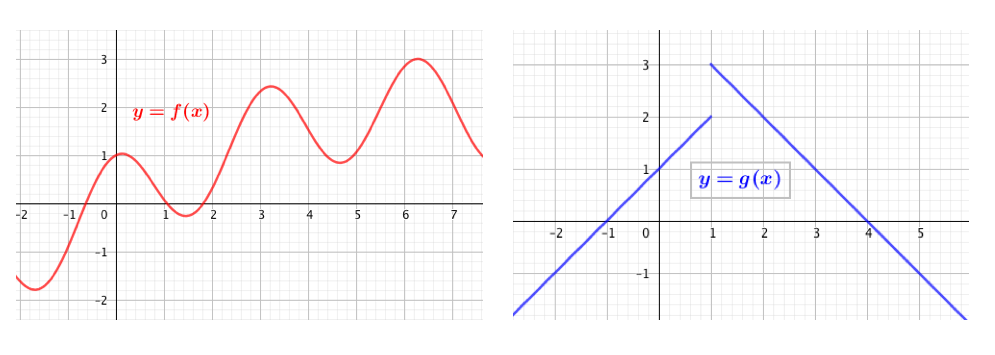
\includegraphics[width=1\textwidth]{imagenes/imagenes03/T03IM09.png}
			\caption{$f$ es continua, pero $g$ no lo es.}
		\end{figure}
	
	La \emph{continuidad}, en matemáticas, es una \emph{condición local}, es decir, una función es o no continua en un punto. Después extenderemos el concepto de continuidad a un intervalo diciendo que la función será continua en él si lo es en todos los puntos que los forman.
	
	\begin{defi} \label{def-ctndad} Continuidad de una función en un punto.
	
	Decimos que $f(x)$ es continua en $x_0\in Dom(f)$ si $\boxed{ \; \underset{x\to x_0}{lim}\;{f(x)}=f(x_0)\; }$ , es decir, 
	
	si $\forall \varepsilon>0, \exists \delta>0: 0<|x-x_0|<\delta \to |f(x)-f(x_0)|<\varepsilon$
		
	\end{defi}

	Esta definición, a la hora de aplicarla en la práctica al estudio de la continuidad de funciones, se traduce en `\underline{el método de los tres pasos}':
	
	$f(x)$ continua en $x_0$ si:
	
	\hspace{10mm} 1) $\exists f(x_0)$

	\hspace{10mm} 2) $\exists \underset{x\to x_0}{lim}\;{f(x)}$	
	
	\hspace{10mm} 3) $f(x_0)=\underset{x\to x_0}{lim}\;{f(x)}$
	
	\begin{defi}Discontinuidades.
	
	Si $f(x)$ no es continua en $x_0$, decimos que es `discontinua' en él.
	
	\vspace{4mm}TIPOS DE DISCONTINUIDADES: Aunque existen varios tipos de clasificar las discontinuidades según autores distintos, daremos como discontinuidades la siguiente clasificación:
	
	\begin{itemize}
		\item Discontinuidad evitable: $\exists f(x_0);\; \exists \underset{x\to x_0}{lim}\;{f(x)}; \mbox{ pero }f(x_0)\neq\underset{x\to x_0}{lim}\;{f(x)}$
		\item Discontinuidad de salto (finito): $\nexists \underset{x\to x_0}{lim}\;{f(x)} \mbox{ porque } \underset{x\to x_0^-}{lim}\;{f(x)}\neq \underset{x\to x_0^+}{lim}\;{f(x)}$. 
		
		Es decir, los límites laterales existen ambos, son finitos, pero distintos.
		\item Discontinuidad asintótica: $\underset{x\to x_0}{lim}\;{f(x)}=\infty$
		\item Discontinuidades de segunda especie: otros casos distintos a los anteriores.
	\end{itemize}
		
	\end{defi}

	\begin{figure}[H]
		\centering
		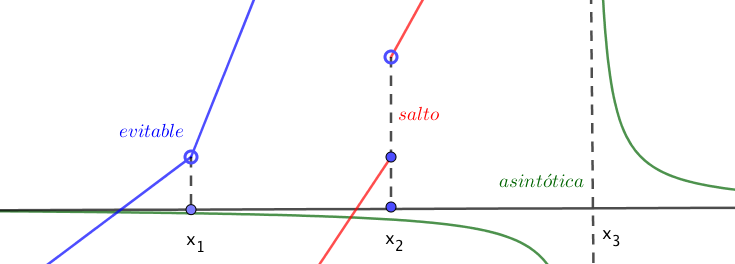
\includegraphics[width=0.7\textwidth]{imagenes/imagenes03/T03IM10.png}
		\caption{Tipos de discontinuidades.}
	\end{figure}

	\begin{defi}Continuidad lateral.
	
		$f(x)$ es continua por la derecha en $x_0$ si $\underset {x\to x_0^+}{lim}\;{f(x)}=f(x_0)$
		
		$f(x)$ es continua por la izquierda en $x_0$ si $\underset {x\to x_0^-}{lim}\;{f(x)}=f(x_0)$
		
	\end{defi}

	\begin{defi}Continuidad en un intervalo.
	
	$f(x)$ es continua en un intervalo abierto $]a,b[$ si lo es $\forall x \in ]a,b[$
	
	$f(x)$ es continua en un intervalo cerrado $[a,b]$ si lo es en el intervalo abierto $]a,b[$ y es continua por la derecha en $a$ y continua por la izquierda en $b$
		
	\end{defi}
	
	\subsection{Continuidad de las funciones elementales}
	
	\begin{teor} Álgebra de funciones continuas.
	
	Sean $f$ y $g$ dos funciones continuas en $x_0$, entonces, las siguientes combinaciones son continuas en $x_0$:
	
	\begin{enumerate}
		\item Sumas: $f+g$
		\item Restas: $f-g$
		\item Productos $f\cdot g$
		\item Producto por constantes: $k\cdot f; \quad \forall k\in \mathbb R$
		\item Cocientes: $f/g$, siempre que $g(x_0)\neq 0$
		\item Potencias: $f^{r/s}$, con $r$ y $s$ enteros y f definida en un intervalo que contenga a $x_0$
		\item Composición: si $f$ continua en $x_0$ y $g$ continua en $f(x_0) \to f\circ g$ continua en $x_0$ 
	\end{enumerate}
		
	\end{teor}

	\begin{proof}
		Demostraremos, p.e., la primera de las propiedades:
		
		$\underset {x\to x_0}{lim}\; {(f+g)(x)}=\underset {x\to x_0}{lim}\; {(f(x)+g(x))}=\underset {x\to x_0}{lim}\; {f(x)}+\underset {x\to x_0}{lim}\; {g(x)} =f(x_0)+g(x_0)=(f+g)(x_0)$ Lo que prueba que $(f+g)$ es continua en $x_0$.
	\end{proof}
	
	\vspace{4mm}Continuidad de funciones elementales:
	\begin{itemize}
		\item Las funciones polinómicas son continuas en todo $\mathbb R$
		\item Las funciones racionales son continuas en su dominio. Presentarán discontinuidades cuando se anule el  denominador.
		\item Las funciones radicales son continuas en sus dominios de definición.
		\item Las funciones $\sin x$ y $\cos x$ y sus combinaciones son continuas en todo $\mathbb R$
		\item La función $\tan x$ presenta discontinuidades asintóticas en $x=(2k+1)\dfrac {\pi}{2},\; \forall k\in \mathbb Z$
		\item La función exponencial es siempre continua.
		\item La función logarítmica es continua en su dominio.
	\end{itemize}
	
	\subsection{Asíntotas}
	\label{subsec-asintotas}
	
	Las asíntotas responden del comportamiento infinito de una función en un punto, son las llamadas \emph{asíntotas verticales}. Independientemente de éstas, otras asíntotas responden del comportamiento finito o infinito de una una función en el infinito, son las llamadas \emph{asíntotas horizontales u oblícuas}.
	
	\begin{defi}.
	
	\begin{itemize}
		
		\item Asíntota Vertical (AV): Decimos que $x=x_0$ es AV de $f(x)$ si $\underset{x\to x_0}{lim}\;{f(x)}=\infty$. Suelen ser valores que anulan el denominador de la función.
		
		Independientemente de que existan o no AV, llamamos:
		
		\item Asíntota Horizontal (AH): Decimos que la recta horizontal $y=b\in \mathbb R$ es AH de $f(x)$ si $\underset{x\to \infty}{lim}\;{f(x)}=b$
		
		En el caso de que no existan AH, puede que la función en el infinito se comporte según una recta oblícua, $y=mx+n$, donde $m$ y $n$ se calculan como se indica a continuación:
		
		\item Asíntota Oblícua (AO) [ si no hay AH]: Decimos que la recta $y=mx+n$ es AO de $f(x)$ si $\underset{x\to x_0}{lim}\;{\dfrac {f(x)} {x} }=m\in \mathbb R$ y $\underset{x\to x_0}{lim}\;{(f(x)-mx)}=n \in \mathbb R$
	\end{itemize}
		
	\end{defi}
	
	Los polinomios no tienen ningún tipo de asíntota.
	
	Una función puede tener ninguna, una, varias, incluso infinitas asíntotas verticales ($y=\tan x$) y las funciones jamás podrán cortar a las asíntotas verticales. En cambio, las funciones pueden tener o no asíntotas horizontales u oblícuas, solo una de ellas o ninguna (aunque pueden ser dos distintas cuando $x\to +\infty$ o $x\to -\infty$) y la función puede cortarla en múltiples ocasiones.

	\begin{figure}[H]
			\centering
			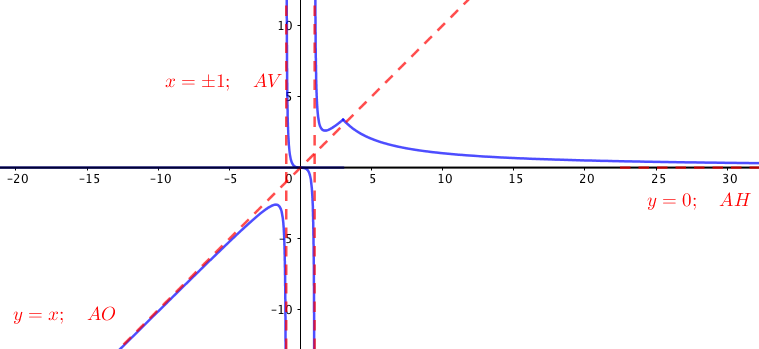
\includegraphics[width=0.75
			\textwidth]{imagenes/imagenes03/T03IM15.png}
		\end{figure}
	
	
	\section{Ejercicios de continuidad}
	\subsection{Ejercicios resueltos de continuidad}
	
	
	
	\begin{ejre} Clasifica las discontinuidades de la  función:  $f(x)=\dfrac {x^3-2x^2+x-2}{x^2-x-2} $
		
	\end{ejre}
	
	\begin{proofw}\renewcommand{\qedsymbol}{$\diamond$}
	
	$x^2-x-2=0 \to x=-1 \wedge x=2$
	
	\begin{itemize}
		\item Continuidad en x=2:
		
		$1) \quad \nexists f(2)=0/0$
		
		$2) \quad \underset{x\to 2}{lim}\; {f(x)}=[0/0;\; mbox{ind.}] =\underset{x\to 2}{lim}\; {\dfrac {(x^2+1)\cancel{(x-2)}}{(x+1)\cancel{(x-2)}}}=\underset {x\to 2}{lim}\; {\dfrac {x^2+1}{x+1}}=5/2$
		
		$3) $ no coinciden
		
		Luego $f(x)$ en $x=2$ es \emph{discontinua evitable}.
		
		\item Continuidad en $x=-1$
		
		$1)\quad \nexists f(1)=-6/0$
		
		$2) \quad \underset {x\to -1}{lim}\; {f(x)}=-6/0=\infty$
		
		$3) $ no coinciden
		
		Luego $f(x)$ en $x=-1$ presenta una \emph{discontinuidad asintótica}.
		\item $\forall x\in \mathbb R \sim \{-1,2 \}$, la función es continua.
	
	\end{itemize}
		
	\end{proofw}
	
	\begin{ejre} Calcula las continuidad de $f(x)=\left\{ \begin{matrix} \dfrac{x+2}{x^2-4} & x\neq -2 \\ k & x=-2 \end{matrix} \right. $
		
	\end{ejre}
	
	\begin{proofw}\renewcommand{\qedsymbol}{$\diamond$}
	
	Hemos de estudiar la continuidad en el nexos de la función, $x=-2$ y, también, en $x=2$ puesto que anula un denominador.
	
	\begin{itemize}
		\item Continuidad en x=2
		
		$1)\quad \nexists f(2)=4/0$
		
		$2)\quad \underset {x\to 2}{lim}\;{\dfrac {x+2}{x^4-4}}=4/0=\infty$
		
		$3)$ no coinciden
		
		$f(x)$ en $x=2$ tiene una \emph{discontinuidad asintótica}
		
		\item Continuidad en $x=-2$
		
		$1)\quad f(-2)=k$
		
		$2) \quad \underset {x\to -2}{lim}\;{\dfrac {x+2}{x^4-4}}=[0/0 \mbox{ind}]=\underset {x\to -2}{lim}\;{\dfrac {\cancel{(x+2)}}{\cancel{(x+2)}(x-2)}}=\underset {x\to -2}{lim}\;{\dfrac {1}{x-2}}=-1/4$
		
		$3) \quad $ si $k=-1/4$, $f(x)$ \emph{continua} en $x=-2$, pero si $k\neq -1/4$, entonces $f(x)$ tendrá una \emph{discontinuidad evitable} en $x=-2$
		
	\end{itemize}
		
	\end{proofw}
	
	\begin{ejre} Calcula la continuidad de $f(x)=\dfrac {x}{\ln (x-2)}$
		
	\end{ejre}
	
	\begin{proofw}\renewcommand{\qedsymbol}{$\diamond$}
	
	Es fácil comprobar que $Dom(\ln (x-2))=]2,+\infty[$, pero el denominador se anula cuando $\ln(x-2)=0 \to x-2=e^0=1 \to x=3$. Hemos, pues, de estudiar la continuidad en x=3, en el resto del domino, la función es continua.
	
	$1)\quad \nexists f(3)=3/0$
	
	$2)\quad \underset {x\to 3}{lim}\; {f(x)}=3/0=\infty$
	
	$3) $ no coinciden, $f(x)$ en $x=3$ tiene una \emph{discontinuidad asintótica}.
	
	Luego $f(x)$ es ctna. $\forall x \in ]2,+\infty[\, \sim \{3\}$, presentando en $x=3$ una discontinuidad asintótica. 
	
		
	\end{proofw}
	
	
	\begin{ejre} Estudia la continuidad de $f(x)=\left\{ \begin{matrix} 
	|x+2| & x<-1 \\ 
	x^2 & -1\le x < 1 \\
	2x+1 & x>1 
	\end{matrix} \right. $	
	\end{ejre}

	\begin{proofw}\renewcommand{\qedsymbol}{$\diamond$}
	
	$f(x)=\left\{ \begin{matrix} 
	|x+2| & x<-1 \\ 
	x^2 & -1\le x < 1 \\
	2x+1 & x>1 
	\end{matrix} \right. = 
	\left\{ \begin{matrix} 
	-x-2 & x<-2 \\
	x+2 & -2\le x<-1 \\ 
	x^2 & -1\le x < 1 \\
	2x+1 & x>1 
	\end{matrix} \right.$

		Puesto que no hay ningún denominador que se anule, solo hemos de estudiar la continuidad en los nexos de la función: $x=\{-2, -1, 1 \}$. En el resto de números reales la función es continua.
		
		\begin{itemize}
			\item Continuidad en $x=-2$
			
			$1) \quad \exists f(-2)=(-2)+2=0$
			
			$2) \quad \exists \underset{x\to -2^-}{lim}\;{f(x)}= \underset{x\to -2^-}{lim}\;{-x-2}=-(-2)-2=0;\qquad \exists \underset{x\to -2^+}{lim}\;{f(x)}= \underset{x\to -2^+}{lim}\;{x+2}=(-2)2=0 \quad \Rightarrow \quad \exists \underset{x\to -2}{lim}\;{f(x)}=0$
			
			$3) $ Coinciden, luego $f(x)$ es \emph{continua} en $x=-2$
			
			\item Continuidad en $x=-1$ 
			
			$1)\quad f(-1)=(-1)^2=1$
			
			$2) \quad \underset {x\to -1^-}{lim}\; {x+2}=-1+2=1; \qquad \underset {x\to -1^-}{lim}\; {x^2}=(-1)^2=1 \quad \Rightarrow \quad \exists \underset{x\to -1}{lim}\;{f(x)}=1$
			
			$3) $ Coinciden, luego $f(x)$ es \emph{continua} en $x=-1$
			
			\item Continuidad en $x=1$
			
			$1)\quad \nexists f(1)$
			
			$2) \quad \underset {x\to 1^-}{lim}\; {x^2}=1; \qquad \underset {x\to 1^+}{lim}\; {2x+1}=3 \quad \Rightarrow \quad \nexists \underset{x\to 1}{lim}\;{f(x)}$ Los límites laterales son finitos y distintos.
			
			$3) $ No coinciden. $f(x)$ tiene una \emph{discontinuidad de salto} en $x=1$
			
			
		\end{itemize}
		
	
	\end{proofw}
	
	\begin{ejre}Estudia las asíntotas de $f(x)=\dfrac {3x-1}{x+2}$
		
	\end{ejre}
	
	\begin{proofw}\renewcommand{\qedsymbol}{$\diamond$}
		
		$\underset {x\to -2}{lim}\;{\dfrac {3x-1}{x+2}}=-7/0=\infty \to x=-2$ AV
		
		$\underset {x\to \infty }{lim}\;{\dfrac {3x-1}{x+2}}=3\to y=3$ AH (luego $\nexists$ AO) 
		
	\end{proofw}

	\begin{ejre} Estudia las asíntotas de $f(x)=\dfrac {x^3+4x^2}{x^2+1}$
		
	\end{ejre}
	
	
	\begin{proofw}\renewcommand{\qedsymbol}{$\diamond$}
	
	$\nexists x_0 \; / \; \underset {x\to x_0}{lim}\;{f(x)}=\infty$, ya que $x^2+1\neq 0, \; \forall x$. Luego $\nexists$ AV
	
	$\underset {x\to \infty}{lim}\;{f(x)}=\infty$, ya que el numerador es de grado mayor al denominador, por ello $\nexists$ AH. Veamos si $\exists$ AO: $y=mx+n$
	
	$m=\underset {x\to \infty}{lim}\;{\dfrac {f(x)}{x}}=\underset {x\to \infty}{lim}\;{\dfrac {x^3+4x^2}{x^3+x}}=1$. 
	
	Busquemos ahora $n=\underset {x\to \infty}{lim}\;{\left(\, f(x)-1\cdot x \right)}=\underset {x\to \infty}{lim}\;{ \left( \dfrac {x^3+4x^2}{x^2+1}-x \right) }=\underset {x\to \infty}{lim}\;{\dfrac {4x^2-x}{x^2+1}=4}\to $ 
	
	$\to y=x+4$ es la AO.
		
	\end{proofw}
	
	\begin{ejre} Estudia las asíntotas de $f(x)=\dfrac {x^4}{x^2+1}$
		
	\end{ejre}
	
	\begin{proofw}\renewcommand{\qedsymbol}{$\diamond$}
	
	Como $x^2+1\neq 0 \to \nexists$ AV
	
	Como $\underset {x\to \infty}{lim}\;{f(x)}=\infty \to \nexists $ AH
	
	Como $\underset {x\to \infty}{lim}\;{\dfrac {f(x)}{x}}=\underset {x\to \infty}{lim}\;{\dfrac {x^4}{x^3+x}}=\infty \to \nexists m \to \nexists $ AO
	
	Esta función no tiene ningún tipo de asíntota.
	
	\end{proofw}
	
	
	
	\begin{ejre} Calcula las asíntotas de la función $f(x)=\sqrt{
	x^2-2x}$
		
	\end{ejre}
	
	\begin{proofw}\renewcommand{\qedsymbol}{$\diamond$}
	
	Es fácil comprobar que la función no tiene ni asíntotas verticales ni horizontales y que su dominio es $]-\infty,0]\cup[2,\infty[$. Veamos pues sus asíntotas oblícuas, en plural, porque la raíz puede tener comportamiento distinto en $\pm \infty$.
	
	*  AO cuando $x\to +\infty$: $\quad y=mx+n$
	
	$m=\underset {x\to +\infty}{lim}\; {\dfrac {\sqrt{x^2-2x}}{x}}=1$; $\quad n=\underset {x\to +\infty}{lim}\; {(\sqrt{x^2-2x}-x)}=[\infty - \infty: \mbox{conjugado}]= \underset {x\to +\infty}{lim}\; {\dfrac {-2x}{\sqrt{x^2-2x}+x}}=\dfrac {-2}{1+1}=-1$; $\qquad y=x-1:$ AO ($x\to +\infty$).
	
	\vspace{3mm}* AO cuando $x\to -\infty$: $\quad y=mx+n$
	
	$m=\underset {x\to -\infty}{lim}\; {\dfrac {\sqrt{x^2-2x}}{x}}=[x=-t]=\underset {t\to +\infty}{lim}\; {\dfrac {\sqrt{t^2+2t}}{-t}}=-1$; $\quad n=\underset {x\to -\infty}{lim}\; {(\sqrt{x^2-2x}+x)}=
	[x=-t]=\underset {t\to +\infty}{lim}\; {(\sqrt{t^2+2t}-t)}=[\infty - \infty: \mbox{conjugado}]= \underset {t\to +\infty}{lim}\; {\dfrac {2t}{\sqrt{t^2+2t}+t}}=\dfrac {2}{1+1}=1$; $\qquad y=-x+1:$ AO ($x\to -\infty$).
	
	
		
	\end{proofw}
	
		
	\begin{ejre} Calcula las asíntotas de $f(x)=\dfrac {|x|}{x+1}$
		
	\end{ejre}
	
	\begin{proofw}\renewcommand{\qedsymbol}{$\diamond$}
	
	Obviamente, $f(x)$ es una función definida a trozos:
	
		\begin{equation*}
		f(x)=
		\begin{cases} 
		\;\;  \dfrac {-x}{x+1} &\mbox{si } x< 0 \\ 
		\; \dfrac {x}{x+1} & \mbox{si } x \ge 0 
		\end{cases}
		\end{equation*}
		
		$\underset {x\to -1}{lim}\; {f(x)}= \underset {x\to -1}{lim}\; {\dfrac {-x}{x+1}}=-1/0=\infty \qquad x=-1$: AV
		
		$\underset {x\to +\infty}{lim}\;{f(x)}= \underset {x\to +\infty}{lim}\;{\dfrac {x}{x+1}}=1 \qquad y=1$: AH $(x\to +\infty)$
		
		$\underset {x\to -\infty}{lim}\;{f(x)}= \underset {x\to -\infty}{lim}\;{\dfrac {-x}{x+1}}=[x=-t]=\underset {t\to +\infty}{lim}\;{\dfrac {t}{-t+1}}=-1 \qquad y=-1$: AH $(x\to -\infty)$
		
		
		
	\end{proofw}
	
	\begin{ejre} Demostrar que la función de Diriclhet (figura \ref{fig:dirichlet}) no es continua en ningún punto.
	
	\begin{equation*}
		f(x)=
		\begin{cases} 
		\;\;  0 &\mbox{if } x \in \mathbb{Q} \\ 
		\; 1 & \mbox{if } x \in \mathbb{R} \sim \mathbb{Q} 
		\end{cases}
		\end{equation*}
		
	\end{ejre}

	\begin{proofw}\renewcommand{\qedsymbol}{$\diamond$}
		
		Sea $x_0 \in \mathbb Q$, siempre podemos construir una sucesión de números irracionales $ \{ \alpha_n \} \to x_0$, pero entonces, al acercarnos a $x_0$ con estos números irracionales, $f(\alpha_n)=1, \; \forall n$, al ser $\alpha_n$ irracionales. es decir: $\underset{\alpha_n \to x_0}{lim}\;{f(x)}=1\neq f(x_0)=0$, por ser $x_0$ racional. Luego $f(x)$ no puede ser continua en ningún número racional.
		
		Sea $x_1 \in \mathbb R \sim \mathbb Q$, siempre podemos construir una sucesión de números racionales $ \{ \beta_n \} \to x_1$, pero entonces, al acercarnos a $x_1$ con estos números racionales, $f(\beta_n)=0, \; \forall n$, al ser $\beta_n$ racionales. es decir: $\underset{\beta_n \to x_1}{lim}\;{f(x)}=0\neq f(x_1)=1$, por ser $x_1$ irracional. Luego $f(x)$ no puede ser continua en ningún número iracional.
		
		Conclusión: f(x) no es continua en ningún número real.
		
	\end{proofw}

	
	
	
	
	\subsection{Ejercicios propuestos de continuidad}
	
	\emph{Los ejercicios de cálculo de asíntotas los dejaremos para cuando estudiemos el tema de `representación gráfica de funciones explícitas'.}
	
		\begin{enumerate}[1).-  ]
		
		\item Estudia la continuidad de $f(x)=\dfrac {x^3-2x^2-3x}{x^2-x-6}$
		
		\rightline{\textcolor{gris}{Solución: $x=-2$ asintótica; $x=3$ evitable.}}
		
		\item Calcula las continuidad de $f(x)=\left\{ \begin{matrix} e^{1-x^2} & x\le -1 \\ -\dfrac 1 x & x>-1 \end{matrix} \right. $
		
		\rightline{\textcolor{gris}{Solución: $x=-1$, salto; $x=0$, asintótica}}
		
		\item Calcula el valor de $\quad k \quad$ para que la siguiente función sea continua en todo $\mathbb R$  $\qquad f(x)=\left\{ \begin{matrix} \dfrac{x^3-1}{x-1} & x\neq 1 \\ \ln k & x=1 \end{matrix} \right. $
		
		\rightline{\textcolor{gris}{Solución: $k=e^3$}}
		
		\item Estudia la continuidad de las funciones siguientes:
		
		$a)\quad  f(x)=\left\{ \begin{matrix} e^x & x< 1 \\ \ln x & x\ge1 \end{matrix} \right. $ $\qquad \qquad b)\quad  f(x)=\left\{ \begin{matrix} \dfrac 1 x & x< 1 \\  2x-1 & x\ge1 \end{matrix} \right. $ 
		
		\rightline{\textcolor{gris}{Solución: $a)\quad x=1 \mbox{ salto; }\qquad b) \quad x=0 \mbox{ asintótica; } x=1 \mbox{ continua.}$}}
		
		\item La siguiente función es continua en $]-1,+\infty[$, halla el valor de $a$
		 
		 $f(x)=\left\{ \begin{matrix} x^2-4x+3 & -1<x<0 \\ \dfrac{x^2+a}{x+1} & x\ge0 \end{matrix} \right. $
		 
		 \rightline{\textcolor{gris}{Solución: $a=3$}}
		 
		 \item Calcula el valor de $t$ para que la siguiente función sea continua en $x=2$.
		 
		 $f(x)=\left\{ \begin{matrix} 
		|x-1|-t & x\le -2 \\ 
		x-5 & x>2  
		\end{matrix} \right.$

		\rightline{\textcolor{gris}{Solución: $t=4$}}
		
		\item Encuentra los valores de $a$ y $b$ para que la siguiente función sea continua y si gráfica pase por el origen de coordenadas.
		 
		 $f(x)=\left\{ \begin{matrix} 
		\ln x - 1 & x>1 \\ 
		2x^2+ax+b & x\le 1  
		\end{matrix} \right.$

		\rightline{\textcolor{gris}{Solución: Ayuda, pasar por el origen supone que si $x=0 \to y=0\quad a=3;\; b=0$}}
		
		\item Encuentra los valores de $a$ y $b$ para que la siguiente función sea continua en $\mathbb R$ y pase por el punto $(-1,2)$.
		 
		 $f(x)=\left\{ \begin{matrix} 
		ax^2+b & |x|\le 2 \\ 
		\dfrac {1}{x^2} & |x|>2  
		\end{matrix} \right.$

		\rightline{\textcolor{gris}{Solución:  $a=3/4;\; b=-11/4$}}
		
		
		\item Encuentra el valor de $m$ para que la siguiente función tenga límite finito en $x=3/2$ y calcula su valor:
		$f(x)=\left\{ \begin{matrix} 
		\dfrac {9-mx^2}{3-2x} & x\neq 3/2 \\ 
		1 & x=3/2  
		\end{matrix} \right.$
		
		\rightline{\textcolor{gris}{Solución:  $m=4;\; \mbox{límite}=6$}}
		
		\item .
		
		\begin{figure}[H]
			\centering
			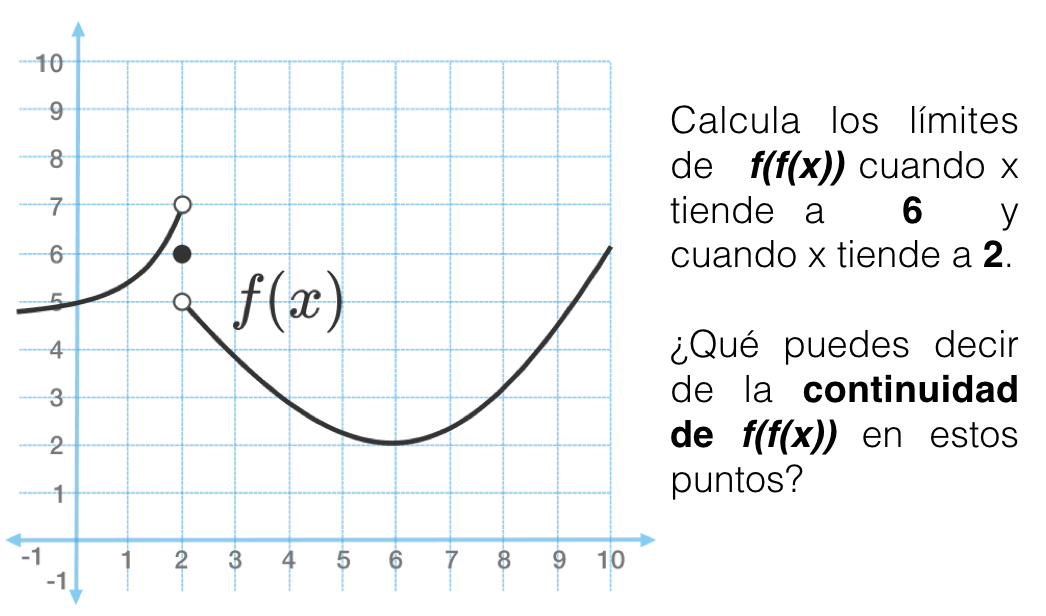
\includegraphics[width=0.75
			\textwidth]{imagenes/imagenes03/T03IM11.png}
		\end{figure}
		
		\rightline{\textcolor{gris}{Solución:  $f(f(6^-))=f(2^+)=5; \quad f(f(6^+))=f(2^+)=5; \quad f(f(6))=6 \quad \mbox{evitable}$}}
		\rightline{\textcolor{gris}{  $f(f(2^-))=f(7^-)=2.5; \quad f(f(2^+))=f(5^-)=2.5; \quad f(f(2))=2 \quad \mbox{evitable}$}}
		
		\item Calcula las asíntotas de a) $f(x)=\dfrac {x^3-x^2+1}{2x^2-x+3} \qquad$ b) $f(x)=\dfrac {x^5+2x^2-5}{x^4-1}$
		
		\rightline{\textcolor{gris}{Solución: a) $y=\frac 1 2 x-\frac 1 4 \quad $ b) $x=\pm 1; \; y=x$ }}
		
		\item Calcula las asíntotas de a) $f(x)=\dfrac {\sqrt{1-x}}{3x} \qquad$ b) $f(x)=\dfrac {x+\sqrt{x^2+1}}{x}$
		
		\rightline{\textcolor{gris}{Solución: a) $x=0; \; y=0 \; (x\to -\infty) \quad$ b) $x=0; \; y=2 \; (x\to +\infty); \; y=0 \; (x\to -\infty)$}}
		
		\item Calcula las asíntotas de a) $y=\ln{\dfrac {x^2-1}{x^2+1}}\qquad$ b) $y= \dfrac {e^x-1}{e^x+1}$
		
		\rightline{\textcolor{gris}{Solución: a) $x=\pm 1; \; y=0\quad$ b)$\nexists AV; \; y=\pm 1 \; (x\to \pm \infty)$ }}
		
		\item Calcula las asíntotas de a) $y=\ln \dfrac {x}{x+1}\qquad$ b) $y=\dfrac {e^{|x-1|}}{x^2+2x-3}$
		
		\rightline{\textcolor{gris}{Solución: a) $x=1^-;\; x=0^+; \; y=0 \quad$ b) $x=-3; \; x=1; \; \nexists AH; \; \nexists AO$}}
		
		\item Considera la función $f(x)=\dfrac {ax+8}{bx+6}$. Encuentra los valores de $a$ y $b$ para que las rectas $x=2$ e $y=-4$ sean, respectivamente, su asíntota vertical y horizontal.
		
		\rightline{\textcolor{gris}{Solución $a=12;\quad b=-3$ }}
		
		\item Hallar $a$ y $b$ para que la siguiente función sea continua en todo $\mathbb R$.
		
		$f(x)=
		\begin{cases}
		a(x-1)2 & \mbox{ si } x\le 0 \\	
		\sin (b+x) & \mbox{ si } 0<x<\pi \\	
		\dfrac \pi x & \mbox{ si } x\ge \pi 
		\end{cases}
		$
	
		\rightline{\textcolor{gris}{Solución: $a=-1; \; b=\dfrac {3\pi}{2}+2k\pi,\; k\in \mathbb Z$ }}
		
		\item Hallar $a$ y $b$ para que la siguiente función sea continua en todo $\mathbb R$.
		
		$f(x)=
		\begin{cases}
		a \; e^{ \dfrac {\sin^2 x}{x} }+b \cos x & \mbox{ si } x< 0 \\	
		6 & \mbox{ si } x=0 \\	
		3a \; \dfrac {\sin x}{x}+b(x-1) & \mbox{ si } x>0 
		\end{cases}
		$
		
		\rightline{\textcolor{gris}{Solución:$a=b=3$}}
		
		\item Estudia la continuidad de la función: $f(x)=\dfrac {e^x}{x^2+k}$
		
		\rightline{\textcolor{gris}{Solución:Si $k>0$, $f$ comtinua en todo $\mathbb R$;}}
		
		\rightline{\textcolor{gris}{Si $k\le 0$, f tiene discont. asintóticas en $x=\pm \sqrt{-k}$ }}
		
		\item Estudia la continuidad de la función: $f(x)=
		\begin{cases}
		1 & \mbox{ si } x=0\\	
		\dfrac {|\sin x|}{x} & \mbox{ si } x \neq 0
		\end{cases}$
		
		\rightline{\textcolor{gris}{Solución:$f$ discontinua de salto en $x=0$ }}
		
		\item Dada la función:  $f(x)=\dfrac {|x-2|}{|x-1|-1}$,
		
		$a) \quad $ Define la función a trozos.
		
		$b) \quad $ Estudia su continuidad.
		
		\rightline{\textcolor{gris}{Solución: hay que romper la función como aprendimos en el ejercicio \ref{ejre:rompe-trozos}.}}
		\rightline{\textcolor{gris}{El denominador se anula para $x=2$ y para $x=0$}}
		\rightline{\textcolor{gris}{$f(x)= \dfrac {x-2}{2} \quad \ si \quad x<1$ }}
		\rightline{\textcolor{gris}{$f(x)=-1 \quad si \quad 1\le x < 2 \sim \{0\}$}}
		\rightline{\textcolor{gris}{$f(x)=1 \quad si \quad x>2$}}
		\rightline{\textcolor{gris}{Continua en $x=1$; discontinua de salto en $x=2$; discontinua asintótica en $x=0$}}
		
		\item Calcula $a$ y $b$ para que la siguiente función sea continua en $\mathbb R$
		
		$f(x)=
		\begin{cases}
		\dfrac 1 {e^x} & \mbox{ si } x\le 0 \\	
		a\; \cos x + b & \mbox{ si } 0< x \le \pi \\
		\sin x - a\; x & \mbox{ si } x> \pi 
		\end{cases}$
	
		\rightline{\textcolor{gris}{Solución: $a=\dfrac 1 {2(\pi - 1)}; \quad b=\dfrac 1 2$}}

		\item Estudia la continuidad de $f(x)=\begin{cases}
		|x+2| & \mbox{ si } 	x<-1 \\
		x^2 & \mbox{ si } 	-1\le x \le 1 \\
		2x+1 & \mbox{ si } 	x>1 
		\end{cases}$ 
		
		\rightline{\textcolor{gris}{Solución: Discontinua de salto en $x=1$}}
	
		\end{enumerate}
		
			
	\section[Propiedades de las funciones continuas en intervalos cerrados] {Propiedades de las funciones continuas en intervalos cerrados \sectionmark{Propiedades funciones continuas}} 
	\sectionmark{Propiedades funciones continuas} 
	
	\label{prop-func-ctnas}


		\begin{figure}[H]
			\centering
			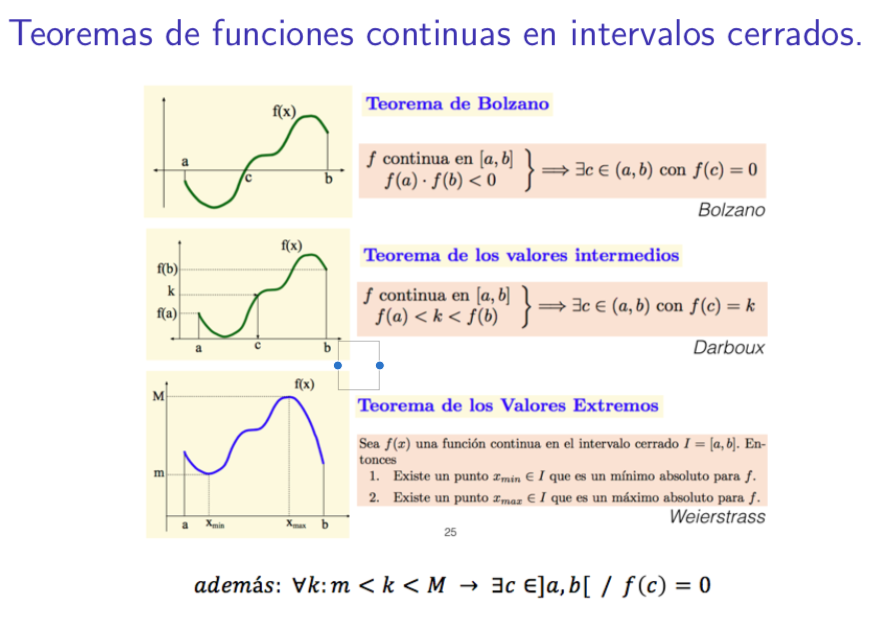
\includegraphics[width=1\textwidth]{imagenes/imagenes03/T03IM12.png}
		\end{figure}
	

	\begin{teor}{Principio de Intervalos Encajados. G. Cantor}.
	
	Sea $I_n$ usa sucesión de intervalos cerrados y encajados, es decir, $I_n=[a_n,b_n];\; I_{n+1}=[a_{n+1},b_{n*1}]$, con $I_{n+1} \subset I_n,; \forall n\in \mathbb N$ y tales que su longitud tiende a cero (se hace cada vez más pequeña): $\underset {n \to +\infty}{lim}\;{long(I_n)} = \underset {n \to +\infty}{lim}\;{(b_n-a_n)} = 0 \quad \Rightarrow \quad \exists \;!\; c\in \mathbb R: \; \underset { n\ge 1 }{ \bigcap  } { \; I_{ n } \; }=\left\{ c \right\} $
		
	\end{teor}
	
	La demostración de este teorema excede de las pretensiones del presente texto y se basa en que toda sucesión monótona y acotada alcanza el supremo o el ínfimo.
	
	
	
	\begin{teor}Teorema de Bolzano: 
		
	
Si f, continua y toma distinto signo en los extremos de un intervalo cerrado, se anula en algún punto intermedio.



 $f : [a,b] \to  \mathbb R,\; continua; \; f(a)\cdot f(b)<0 \Rightarrow \exists \; c \in ]a,b[: \; f(c)=0$ 

	\end{teor}

	\begin{proof}.
	\begin{multicols}{2}
	Dividimos $[a, b]$ por la mitad. Si en el punto medio $f$ vale $0$, hemos concluido. Si no, elegimos, de los dos intervalos en que hemos dividido $[a,b]$ el semiintervalo $[a_1,b_1]$ en cuyos extremos $f$ tiene distinto signo. Lo dividimos de nuevo. . . Repitiendo la operación, obtenemos una sucesión de intervalos encajados $[a_n, b_n]$, de longitud $(b - a)/2n$ que tiende a cero, y , por el \emph{Principio de intervalos encajados de Cantor}, define un punto único $c$ en el que la función es nula. De lo contrario, al ser $f$ continua, $\underset {x\to c}{lim}\; {f (x)} = f (c) \neq 0$ y existirá un entorno de $c$ en el que $f$ toma el signo del límite (Teorema de Conservación del Signo -lema \ref{teor:conserva-signo}-). Pero en todo entorno de $c$ existen puntos en que $f$ es mayor que $0$ y puntos en los que es menor. Entonces, por reducción al absurdo, $f(c) = 0$. 

	\begin{figure}[H]
 		\centering
		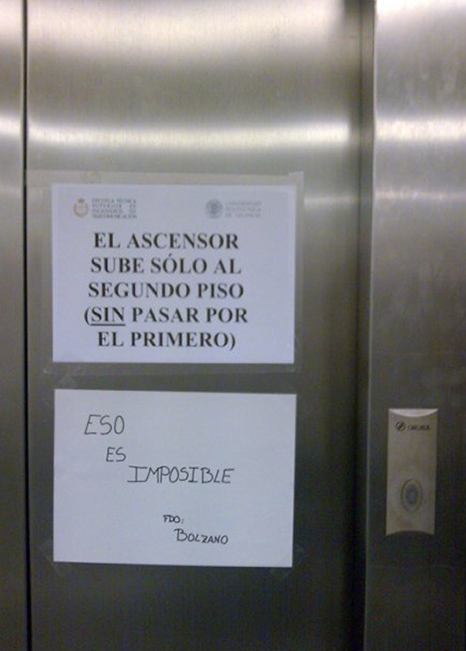
\includegraphics[width=.3\textwidth]{imagenes/imagenes03/xiste03.png}
	\end{figure}
	\end{multicols}

\end{proof}

	OBSERVACIONES SOBRE EL TEOREMA DE BOLZANO:
	
	\begin{itemize}
		\item Geométricamente, el teorema asegura que una curva continua en un intervalo cerrado que tome valores de distinto signo en los extremos del intervalo cortará, al menos una vez, al eje OX.
		\item La condición de continuidad en el intervalo cerrado es totalmente necesaria, sin ella el teorema no tiene por qué cumplirse, como muestra la siguiente figura.
		
		\begin{figure}[H]
 		\centering
			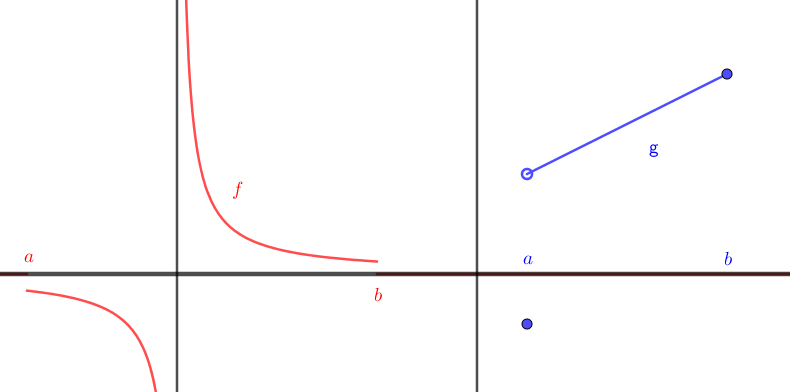
\includegraphics[width=.6\textwidth]{imagenes/imagenes03/T03IM14.png}
			\caption{$f$ no continua en $]a,b[$, tiene una discontinuidad asíntótica en $0\in [a,b]$ ; $g$ no continua en $[a,b]$, discontinua en $a$ por la derecha}
		\end{figure}
		
	\end{itemize}


	\begin{teor} Propiedad de Darboux (del valor intermedio):
	
	 Si $f$, continua en $[a,b]$, tal que toma valores distintos en $a$ y en $b$, entonces toma todos los valores intermedios, al menos una vez, entre $f(a$) y $f(b)$ 
	 
	 $f \mbox{ continua } [a,b], \mbox{supongamos, sin límite de generalidad, que } f(a)<f(b) \rightarrow \forall \; y \; / \; f(a)<y<f(b), \; \exists c \in ]a,b[ : f(c)=y$
	\end{teor}

	\begin{proof}
		
 	Definimos $g(x) = f(x) - y$, que cumple $g(a) < 0, \; g(b) > 0$ $\quad g(a)=f(a)-y <0;\; g(b)=f(b)-y>0 \quad , \mbox{ por hipótesis} $. Entonces, por el teorema de Bolzano, $\exists \; c \in  ]a, b[ \; / \;  g(c) = f (c) - y = 0 \to   f (c) = y$

 	\end{proof}
 


	\begin{teor} Teorema de Weierstrass (o de los valores extremos): 
		
	
	Toda función continua en un intervalo cerrado alcanza en él un máximo y un mínimo. 
	
	\end{teor}
	
	\begin{proof}.
		
	\begin{itemize} 
	
	
	\item [*] $f$ está acotada en $[a, b]$. Supongamos que no. Dividimos $[a, b]$ en dos semiintervalos. Elegimos aquél en que $f$ no está acotada (al menos no lo está en uno de ellos). Lo dividimos de nuevo. . . Repitiendo la operación, obtenemos una sucesión de intervalos encajados que define un punto $\alpha$, tal que $f$ no está acotada en ningún entorno suyo. Pero, al ser $f$ continua, $\underset {x\to \alpha }{lim}\;{f(x)} = f(\alpha)$ y $f$ está acotada en un entorno de  $\alpha$, llegamos a una contradicción.
	
	\item [*] Al ser $f$ acotada en $I = [a, b]$, $f(I)$ tiene supremo $M$ e ínfimo $m$. Veamos que son máximo y mínimo (f los alcanza). En efecto, si $M$ no es alcanzado por $f$, la función $g(x) = \dfrac {1}{M - f(x)}$ será continua en $I$, por lo tanto acotada. Entonces $\exists \; k \; / \;  \dfrac {1}{M-f(x)} < k, \; \forall x \in I \Rightarrow  f(x) < M  - \dfrac 1 k$, y $M$ no sería el supremo. 
	
		Es decir, $x_1,\; x_2 \; \in \;  I \; /\;  f(x1) = m,\;  f(x2) = M $
		
	\end{itemize}

 
 	\end{proof}
 	
	\begin{coro}
 		Una función continua transforma un intervalo cerrado en un intervalo cerrado.
 	\end{coro}
 	
 	\begin{proof}.
 	
 	
 	\begin{itemize}
 		
 	
 	
 	 \item [*] Por el teorema de Weierstrass, $f$ , continua en $[a, b]$, alcanza en él un máximo $M$ y un mínimo $m$.
 	
 	 \item [*] Por la propiedad de Darboux, $f$ alcanzará todos los valores comprendidos entre $m$ y $M$, con lo que $[a, b]$ se transforma en $[m, M]$.
 	 
 	 \end{itemize}
 
 
 	\end{proof}
	
 		\begin{figure}[H]
 		\centering
			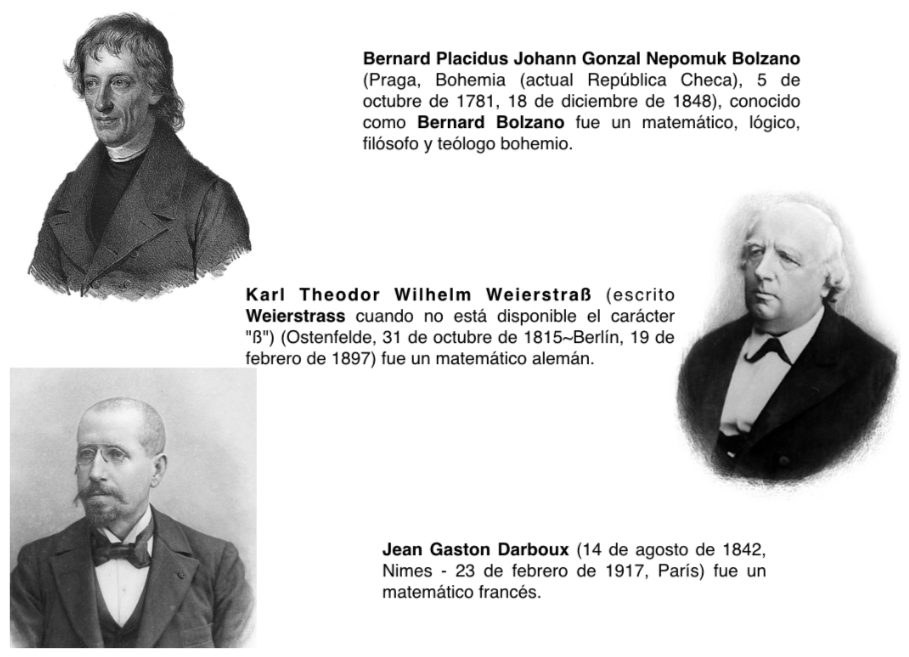
\includegraphics[width=1\textwidth]{imagenes/imagenes03/T03IM13.png}
		\end{figure}
 	
	\section{Ejercicios de teoremas de funciones continuas}
	
	\subsection{Ejercicios resueltos de teoremas de funciones continuas}
	
	
	\begin{ejre} Demuestra que la ecuación $x^3+x^2-2x$ tiene al menos una raíz en el intervalo $[1/2,3/2]$		
	\end{ejre}
	
	\begin{proofw}\renewcommand{\qedsymbol}{$\diamond$}
	
	Definimos $f(x)=x^3+x^2-2x$, que es una función continua en todo $\mathbb R$ por ser polinómica, por lo que es continua en $[1/2,3/2]$. Además, $f(1/2)=-5/8<0$ y $f(3/2)=21/8>0$. Se verifican, pues, las hipótesis del teorema de Bolzano, por lo que $\exists \; c \in [1/2,3/2] \; / \; f(c)=0$, es decir, $\exists \; c \in [1/2,3/2] \; / \; c^3+c^2-2c=0$ y es esa $c$ la raíz buscada.
	\end{proofw}
	
	
	\begin{ejre} ?`Es posible aplicar el teorema del valor intermedio en $[-2,4]$ a la función 		$f(x)=\left\{ \begin{matrix} 
		2x-1 & -2\le x <2 \\ 
		x+4 & 2 \le x \le 4  
		\end{matrix} \right.$ ?
	\end{ejre}
	
	\begin{proofw}\renewcommand{\qedsymbol}{$\diamond$}
		
	

	La función, por ser ambos trozos polimómicos, es continua en todo su dominio excepto, tal vez, en el nexo $x=2$, donde hemos de estudiar la continuidad.
	
	Continuidad en $x=2$
	
	$1)\quad \exists f(2)=2+4=6$
	
	$2)\quad \nexists \underset {x\to 2}{lim}\;{fx}$ porque no coinciden los límites laterales: $\underset{x\to 2^-}{lim}\;{2x-1}=3\neq 6 =\underset{x\to  2^+}{lim}\;{x+4}$
	
	$3) \quad $ no coinciden, f(x) es \emph{discontinua de salto} en $x=2$
	
	Al no ser $f(x)$ continua en $[-2,4]$, no se puede aplicar el teorema del valor intermedio.

	\end{proofw}
	
	\begin{ejre} Determinar si el polinomio $x^4-4x^2-1$ tiene alguna raíz negativa.		
	\end{ejre}
	
	\begin{proofw}\renewcommand{\qedsymbol}{$\diamond$}

	Hemos de encontrar un intervalo en $\mathbb R^-$ en que la función tome valores de distinto signo en sus extremos, ya que continua siempre lo será al ser un polinomio.
	
	Es fácil encontrar que en $[-3,0]$ ocurre lo dicho, $f(0)=-1<0$, $f(-3)=81-36-1=44>0$. Luego se puede aplicar el teorema de Bolzano y seguro que $\exists \; c \in ]-3,0[, \quad c<0;\quad \; / \; f(c)=c^4-4c^2-1=0$ 
	\end{proofw}
	
	\begin{ejre} Prueba que la ecuación $x=\cos x$ tiene solución positiva.		
	\end{ejre}
	
	\begin{proofw}\renewcommand{\qedsymbol}{$\diamond$}
	
	Es fácil encontrar un intervalo en $\mathbb R^+$ en que la función $f(x)=x-\cos x$, que evidentemente es continua, tome valores de distinto signo, p.e. $[0,\pi/2]$. 
	
	$f(0)=0-\cos (0)=0-1=-1<0; \quad f(\pi/2)=\pi/2-\cos(\pi/2)=\pi/2-0=\pi/2>0$. Lo cual prueba que $f(x)$ verifica el teorema de Bolzano en $[0,\pi/2]$, por lo que seguro que $\exists \; c \in ]0,\pi/2[$, es decir, $c>0$, tal que $f(c)=c-\cos(c)=0 \to c=\cos(c)$
	\end{proofw}
	
	
	\begin{ejre} 	Demuestra que existe un punto $x=c$ en el que la función $f(x)=x^2+x\cdot 2^x$ toma el valor $2$. 	
	\end{ejre}
	
	\begin{proofw}\renewcommand{\qedsymbol}{$\diamond$}
	Definimos la función $h(x)=f(x)-2=x^2+x\cdot 2^x - 2$ que es continua en todo $\mathbb R$ y al considerarla en el intervalo $[0,1]$ ocurre que toma valores de distinto signo en los extremos (compruébese) por lo que es susceptible de aplicarle el teorema de Bolzano, que demostraría la tesis que queremos probar.
	
	\end{proofw}
	
	\begin{ejre} 	$\divideontimes$. Suponiendo que la temperatura varía de forma continua, prueba que siempre hay dos puntos antípodas en el ecuador terrestre que están a la misma temperatura. 	
	\end{ejre}
	\begin{proofw}\renewcommand{\qedsymbol}{$\diamond$}
	
	Sea $L$ la longitud del ecuador terrestre (unos cuarenta mil kilómetros). Sea $T:[0,L]\to \mathbb R$	la función que a cada punto $x\in[0,L]$ le hace corresponder su temperatuta $T(x)$, medida en grados centígrados, que hay en dicho punto del ecuador. Suponemos (razonablemente) que $T(x)$ es una función continua. Se trata de probar que hay algún punto $c\in [0,L/2]$ tal que $T(c)=T(c+L/2)$ (lo de $L/2$ es por lo que los puntos han de ser antípodas). Consideremos la función $f(x)=T(x+L/2)-T(x)$, definida en el intervalo $[0,L/2]$. Se tiene que $f(0)=T(0+L/2)-T(0)=T(L/2)-T(0)$ y que $f(L/2)=T(L/2+L/2)-T(L/2)=T(L)-T(L/2)=T(0)-T(L/2)$, Ya que $L=0$, $L$ vuelve a ser el punto de partida pues el ecuador es una curva cerrada. Basta darse cuenta de que $f(0)$ y $f(L/2)$ son opuestos ($f(0)\cdot f(L/2)<0)$ y $f$ continua en $[0,L/2] \Rightarrow$ se cumple el teorema de Bolzano y $\exists \; c \in ]0,L/2[ \; / \; f(c)=0 \to T(c+L/2)-T(c)=0 \to T(c)=T(c+L/2)$, dos puntos antípodas en el ecuador que están a la misma temperatura.
	\end{proofw}

	
	\subsection{Ejercicios propuestos de teoremas de funciones continuas}
	
	
	
	\begin{enumerate}
		\item ?`Se puede asegurar que la función $f(x)=\tan x$ tiene una raíz en $[\pi/4, 3\pi/4]$ ?
		 
		\rightline{\textcolor{gris}{Solución: No, es discontinua en $\pi/2$}}
		
		\item Demuestra que existe al menos un número real que cumple: $\sin x = x-2$
		 
		\rightline{\textcolor{gris}{Solución: Bolzano a $f(x)=x-\sin x-2$ en $[0,\pi]$}}
		
		\item Demuestra que las funciones $f(x)=x\; \sin x$ y $g(x)=\ln x$ se cortan en $[2,3]$
		 
		\rightline{\textcolor{gris}{Solución: Bolzano a $h(x)=f(x)-g(x)$}}
		
		\item Demuestra que las funciones $f(x)=e^x$ y $g(x)=\dfrac 1 x$ se cortan en un $x>0$.
		 
		\rightline{\textcolor{gris}{Solución: Bolzano a $h(x)=f(x)-g(x)$ en $[0.1, 1]$}}
		
		\item ?`Se puede afirmar que $x^3+x^2-7x+1=0$ tiene al menos una solución en $]0,1[$ ? ?`Y en $]-1,0[$ ?
		 
		\rightline{\textcolor{gris}{Solución: Bolzano a $f(x)=x^3+x^2-7x+1=0$ en los intervalos indicados.}}
		\rightline{\textcolor{gris}{En el primer intervalo sí y en el segundo no}}
		
		\item Calcular, con un error menor a una décima, una raíz positiva del polinomio $x^3+x-1$
		 
		\rightline{\textcolor{gris}{Solución: Bolzano a $f(x)=x^3+x-1$ en $[0,1]$.}}
		\rightline{\textcolor{gris}{\tiny{Dividir en intervalo en 10 partes y localizar el cambio de signo.}}}
		\rightline{\textcolor{gris}{\tiny{Proceder así, dividiendo en 10 partes el intervalo en que se}}}
		\rightline{\textcolor{gris}{\tiny{ produzca el cambio de signo, hasta alcanzar la precisión deseada.}}}

		 
		\item Prueba que la función $f(x)=(x-a)^2\cdot (x-b)^2+x$ toma el valor $(a+b)/2$ para algún valor de $x$.
		 
		\rightline{\textcolor{gris}{Solución: Bolzano a $h(x)=f(x)-\dfrac {a+b}{2}$ en $[a,b]$}}
		
		
		\item Sea $f(x)=x\; \sin \left( \dfrac {\pi}{4}\; x  \right)$. Demuestra que $\exists \; \alpha\in ]0,4[: \; f(\alpha)=f(\alpha+1)$
		 
		\rightline{\textcolor{gris}{Solución: $g(x)=f(x+1); \; h(x)=g(x)-f(x), $ Bolzano en $[0,4]$}}
		
		\item La función $f(x)=\tan x\; $ toma valores de distinto signo en $[\pi/4, 3\pi/4]$ y, sin embargo, no se anula en él. ?`Contradice este ejemplo el teorema de Bolzano?
		
			\rightline{\textcolor{gris}{Solución: La función es no es continua en $[\pi/4, 3\pi/4]$, }}
			
			\rightline{\textcolor{gris}{tiene una discontinuidad asintótica en $x=\pi/2=$}}
		
		\item Demostrar que $x^5+x=1$ tiene, al menos, una solución real.
		
		\rightline{\textcolor{gris}{Solución: $f(x)=x^5+x-1$ en $[0,1]$ y Bolzano}}
		
		\item Dada $f(x)=\dfrac {4x-2}{x^2+1}$, demuestra que $\exists c \in ]0,2[\; / \; f(c)=1$
		
		\rightline{\textcolor{gris}{Solución: Considera $g(x)=f(x)-1$ en $[0,2]$ y Bolzano}}
		
		\item ?`Existe algún número real igual a su cubo menos una unidad?
		
		\rightline{\textcolor{gris}{Solución: Define $f(x)=x-(x^3-1)$, en $[0,2]$ y Bolzano}}
		
		
		\item $\divideontimes$. Un automovilista sale el sábado de Valencia a Madrid a las 8h y el domingo regresa de Madrid a Valencia a la misma hora. sabiendo que tardó el mismo tiempo en ambos viajes, prueba que en algún momento del domingo se encontraba a la misma distancia de Valencia que a la que se encontraba el sábado en ese momento.
		
		\rightline{\textcolor{gris}{ \tiny Solución: {$f(t$) distancia a Madrid el sábado, $g(t)$ distancia a Valencia el domingo definida en $[8,T]$,}}}
		\rightline{\textcolor{gris}{\tiny{ $T$ tiempo total del viaje. Aplica Bolzano a $h(t)=f(t)-(F(T)-g(t)$, con $f(T)=$ distancia Valencia-Madrid)}}}
		
		
	\end{enumerate}	
		